%%%%%%%%%%%%%%%%%%%%%%%%%%%%%%%%%%%%%%%%%
% Masters/Doctoral Thesis 
% LaTeX Template
% Version 2.5 (27/8/17)
%
% This template was downloaded from:
% http://www.LaTeXTemplates.com
%
% Version 2.x major modifications by:
% Vel (vel@latextemplates.com)
%
% This template is based on a template by:
% Steve Gunn (http://users.ecs.soton.ac.uk/srg/softwaretools/document/templates/)
% Sunil Patel (http://www.sunilpatel.co.uk/thesis-template/)
%
% Template license:
% CC BY-NC-SA 3.0 (http://creativecommons.org/licenses/by-nc-sa/3.0/)
%
%%%%%%%%%%%%%%%%%%%%%%%%%%%%%%%%%%%%%%%%%

%----------------------------------------------------------------------------------------
%	PACKAGES AND OTHER DOCUMENT CONFIGURATIONS
%----------------------------------------------------------------------------------------

\documentclass[
12pt, % The default document font size, options: 10pt, 11pt, 12pt
%oneside, % Two side (alternating margins) for binding by default, uncomment to switch to one side
english, % ngerman for German
onehalfspacing, % Single line spacing, alternatives: onehalfspacing or doublespacing
%draft, % Uncomment to enable draft mode (no pictures, no links, overfull hboxes indicated)
nolistspacing, % The class file specifying the document structure

\usepackage[utf8]{inputenc} % Required for inputting international characters
\usepackage[T1]{fontenc} % Output font encoding for international characters

\usepackage{mathpazo} % Use the Palatino font by default

\usepackage[backend=bibtex,style=authoryear,natbib=true]{biblatex} % Use the bibtex backend with the authoryear citation style (which resembles APA)

\addbibresource{sources.bib} % The filename of the bibliography

\usepackage[autostyle=true]{csquotes} % Required to generate language-dependent quotes in the bibliography

\usepackage[hashEnumerators,smartEllipses]{markdown}
\usepackage{tikz}
\usepackage[schoo,simplified]{pgf-umlcd}
\usepackage{amsmath}
\usepackage{url}
\usepackage{hyperref}
\usepackage{algorithm} 
\usepackage{algpseudocode} 
\usepackage{wrapfig}
%\usepackage[english]{babel}
\usepackage{csquotes}

\usepackage{floatrow}
\usepackage{subfig}
\renewcommand{\thesubfigure}{\Alph{subfigure}}
\usepackage{graphicx}
\usepackage{parskip}


%----------------------------------------------------------------------------------------
%	MARGIN SETTINGS
%----------------------------------------------------------------------------------------

\geometry{
	paper=a4paper, % Change to letterpaper for US letter
	inner=2.5cm, % Inner margin
	outer=3.8cm, % Outer margin
	bindingoffset=.5cm, % Binding offset
	top=1.5cm, % Top margin
	bottom=1.5cm, % Bottom margin
	%showframe, % Uncomment to show how the type block is set on the page
}

%----------------------------------------------------------------------------------------
%	THESIS INFORMATION
%----------------------------------------------------------------------------------------

\thesistitle{Dynamic memory traces for sequence learning in spiking networks} % Your thesis title, this is used in the title and abstract, print it elsewhere with \ttitle
\examiner{Prof. Dr. Abigail \textsc{Morrison}} % Your examiner's name, this is not currently used anywhere in the template, print it elsewhere with \examname
\supervisor{Barna \textsc{Zajzon}} % Your supervisor's name, this is used in the title page, print it elsewhere with \supname
\degree{} % Your degree name, this is used in the title page and abstract, print it elsewhere with \degreename
\author{Simon \textsc{Michau}} % Your name, this is used in the title page and abstract, print it elsewhere with \authorname
\addresses{} % Your address, this is not currently used anywhere in the template, print it elsewhere with \addressname

\subject{Computer Science} % Your subject area, this is not currently used anywhere in the template, print it elsewhere with \subjectname
\keywords{} % Keywords for your thesis, this is not currently used anywhere in the template, print it elsewhere with \keywordnames
\university{\href{https://www.rwth-aachen.de/}{RWTH Aachen University}} % Your university's name and URL, this is used in the title page and abstract, print it elsewhere with \univname
\department{\href{https://www.informatik.rwth-aachen.de/}{Department of Computer Science}} % Your department's name and URL, this is used in the title page and abstract, print it elsewhere with \deptname
\group{\href{https://www.fz-juelich.de/de/inm/inm-6}{Computation in Neural Circuits Group}} % Your research group's name and URL, this is used in the title page, print it elsewhere with \groupname
\faculty{\href{http://faculty.university.com}{Faculty Name}} % Your faculty's name and URL, this is used in the title page and abstract, print it elsewhere with \facname

\AtBeginDocument{
\hypersetup{pdftitle=\ttitle} % Set the PDF's title to your title
\hypersetup{pdfauthor=\authorname} % Set the PDF's author to your name
\hypersetup{pdfkeywords=\keywordnames} % Set the PDF's keywords to your keywords
}

\begin{document}

\frontmatter % Use roman page numbering style (i, ii, iii, iv...) for the pre-content pages

\pagestyle{plain} % Default to the plain heading style until the thesis style is called for the body content

%----------------------------------------------------------------------------------------
%	TITLE PAGE
%----------------------------------------------------------------------------------------

\begin{titlepage}
\begin{center}

\vspace*{.06\textheight}
{\scshape\LARGE \univname\par}\vspace{0.5cm} % University name
\textsc{\Large Bachelor Thesis}\\[0.25cm] % Thesis type

\HRule \\%[0.4cm] % Horizontal line
{\huge \bfseries \ttitle\par}%\vspace{0.4cm} % Thesis title
\HRule \\[1.25cm] % Horizontal line
 
\begin{minipage}[t]{0.4\textwidth}
\begin{flushleft} \large
\emph{Author:}\\
\authorname % Author name
\end{flushleft}
\end{minipage}
\begin{minipage}[t]{0.4\textwidth}
\begin{flushright} \large
\emph{1$^{st}$ Examiner:}\\
\examname\\
\emph{2$^{nd}$ Examiner:}\\
Prof. Dr. Michael \textsc{Schaub}\\
\emph{Advisor:} \\
\supname\\ % Supervisor name
\end{flushright}
\end{minipage}\\[1.25cm]
 
\vfill

\large \textit{Bachelor thesis in Computer Science}\\%[0.3cm] % University requirement text
\textit{submitted to the}\\[0.4cm]
\groupname\\\deptname\\\univname\\%[2cm] % Research group name and department name
 
\vfill

Aachen, {\large \today}\\[4cm] % Date
%\includegraphics{Logo} % University/department logo - uncomment to place it
 
\vfill
\end{center}
\end{titlepage}

%----------------------------------------------------------------------------------------
%	ACKNOWLEDGEMENTS
%----------------------------------------------------------------------------------------

\begin{acknowledgements}
\addchaptertocentry{\acknowledgementname} % Add the acknowledgements to the table of contents
Writing this thesis has been profoundly interesting and challenging. Over the course of work I had the opportunity to learn much about scientific work and had a glimpse at neuroscience at the FZ Jülich. For this I want to thank Prof. Dr. Abigail Morrison and in particular my advisor Barna Zajzon. Without him this work would not have been possible, as he helped me to overcome many of its obstacles and also with understanding the context and content of my thesis more deeply, while also being very motivating and supportive.
\\
Finally, I also want to thank my friends and family who have supported me during this time and volunteered to proofread this thesis.
\end{acknowledgements}

%----------------------------------------------------------------------------------------
%	LIST OF CONTENTS/FIGURES/TABLES PAGES
%----------------------------------------------------------------------------------------

\tableofcontents % Prints the main table of contents

\listoffigures % Prints the list of figures

%\listoftables % Prints the list of tables


%----------------------------------------------------------------------------------------
%	THESIS CONTENT - CHAPTERS
%----------------------------------------------------------------------------------------

\mainmatter % Begin numeric (1,2,3...) page numbering

\pagestyle{thesis} % Return the page headers back to the "thesis" style

% Include the chapters of the thesis as separate files from the Chapters folder
% Uncomment the lines as you write the chapters

% Chapter Template

\chapter{Introduction} % Main chapter title

\label{Chapter1} % Change X to a consecutive number; for referencing this chapter elsewhere, use \ref{ChapterX}

For a long time, the brain has been the subject of scientific research and has inspired other fields and technologies, including the domain of computer science. In the last decade, the technologies derived from it have grown popular and become a part of everyday life in the form of e.g. artificial neural networks and machine learning. And deeper insights into the brain's functioning have enabled medicine to treat patients more successfully. But despite all this progress, most of its exact inner workings including learning and memory are still largely unknown, although there is a consensus that the plasticity of synapses is the substrate that enables it.\\
For several decades now, the possibilities of gaining insights into this study object through the emerging computational neuroscience have been growing. Computational neuroscience can test, enhance and develop new models that describe biological reality, as well as help neuroscience by providing means of cerebral simulation.\\
One example of this is the study on sequence learning currently conducted by the department of Computational and Systems Neuroscience (INM-6) at the FZ Jülich, which also offered a small part of this work for a group of bachelor theses on different computational models of sequential learning.
This thesis is one of them and is aimed at replicating the learning model from \parencite{klampfl_maass_2013}.
\\ \ \\
In their work, the authors of \parencite{klampfl_maass_2013} modeled so-called pyramidal cells (PCs) - a type of neuron that appears for example in the prefrontal cortex and is assumed to play an important role in cognition \parencite{10.1093/cercor/bhg093} - with added \textit{lateral inhibition} by creating a modified version of liquid computing model. A liquid computing model (also called liquid state machine) implements a spiking neural network by using recurrent connections between nodes (neurons) that transmit temporal signals (spikes) that activate the nodes in a certain way. The name "liquid state machine" comes from the fact that each node has a continuous state instead of a discrete one, and can pass it on to neighboring nodes, similar to waves  \parencite{maass_markram_2004}. Although one might assume so due to the biological context, it has nothing to do with the plasticity (or liquidity) of connections between nodes.
The phenomenon of lateral inhibition which was also mentioned stems from neuroscience and causes a neuron to prevent its neighboring neurons from firing when it is itself active. In biological reality, this is usually realized by inhibitory synapses connected to the neighboring neurons. These PCs in combination with lateral inhibition tend to form so-called Winner-Take-All (WTA) cortical microcircuits.\\
The main goal of the said paper was to demonstrate how memory, learning, and even certain computational abilities can emerge from WTA cell assemblies with spike-timing-dependent plasticity (STDP; explained in \ref{ssec:spike_timing_dependent_plasticity} and \ref{ssec:stdp}) when presented with sequential input patterns. More specifically they postulated three constraints for this behavior \parencite{klampfl_maass_2013}:
\begin{enumerate}
    \item PCs and inhibitory neurons tend to be organized into specific network motifs
    \item synapses between PCs are subject to STDP
    \item neural responses are highly variable (\glqq trial-to-trial variability \grqq)
\end{enumerate}
By replicating the model from this paper its correctness is supposed to be verified while also providing an Open Source version of it that is accessible for further research and modification. In addition, any hidden assumptions made in the description of the original should be uncovered.\\
To do so, after explaining the methods of this work (Section \ref{sec:methods}), this thesis will first briefly discuss the biological backgrounds needed to help understand its content from the perspective of a Computer Scientist in Chapter \ref{Chapter2}. Following up on this in Chapter \ref{Chapter3} the original model of \parencite{klampfl_maass_2013} will be discussed in more detail and the exact model definitions will be laid out and put to inspection. This leads over to the summary of the implementation produced for this thesis (Chapter \ref{Chapter4}), building on the original implementation and pointing out justified alterations and different technical approaches. Finally, the results of both implementations will be compared in Chapter \ref{Chapter5}, followed by a conclusion and an outlook to future work (Chapter \ref{Chapter6}).
% TODO: explain 
%  sequence learning


\section{Methods} \label{sec:methods}
As already mentioned, this replication study should be viewed as part of a group of studies conducted as part of bachelor theses at the INM-6 (Institute for Medicine and Neuroscience, Computation in Neural Circuits group). All these studies have in common that they are implemented using NEST \parencite{nest_3_3} as their simulation framework to be able to compare the studied models in a more simulator-agnostic way.\\
Kindly the authors of \parencite{klampfl_maass_2013} agreed to share the Python 2.7 implementation code of their work, so when the implemented model deviates from the one in the paper, the implemented model is considered here, since it was used to produce the advertised results.\\
To study and understand the original model more closely, the first phase of this thesis was dedicated to replicating the results of the paper using their original code. The learnings of this phase are presented in Chapter \ref{Chapter3}. Along with replicating the results during this phase, it was also decided to add several means of recording and visualizing certain parameters like membrane potentials, spike activity, and synaptic weights, in order to be able to compare the results with those of the later replication of the model to verify its correctness.\\
After getting familiar with the original implementation, the replication phase started. For the model replication NEST 3.3 \parencite{nest_3_3} was initially chosen but later replaced with the most recent development version at the time. 
NEST (\textbf{NE}ural \textbf{S}imulation \textbf{T}ool) is a simulator for spiking neural networks developed by the NEST initiative and is built to simulate various forms of learning and plasticity. While NEST itself is a standalone application operating on a C++ kernel, it is also possible to run it in Python using PyNEST. This program can translate Python commands for NEST. Due to the superior simplicity and readability of Python compared to C++, the PyNEST option was selected for this thesis.\\
As further elaborated later, entirely new neuron and synapse models are needed, which are not provided by NEST natively. To create these models for NEST, the modeling language NESTML \parencite{nestml_5_0_0} was chosen. NESTML creates neuron and synapse models by translating instructions formulated in the NESTML modeling languages syntax to C++ code that integrates with the main NEST kernel. The language was created to make the process of writing custom neuron and synapse models easier and most importantly more accessible since the construction of such models by hand requires a vast knowledge of the NEST kernel in addition to proficiency in C++ programming. Without NESTML this would further restrict users from working with NEST.\\
During the work on implementing the synapse and neuron models from \parencite{klampfl_maass_2013}, it eventually became clear that NESTML was not capable of fulfilling the requirements of the model. For this reason, NESTML could not further be used to create the models. The incomplete generated model implementations of NESTML were however used as the platform to build a highly customized C++ model by hand (described in Section \ref{sec:neuron_synapse_models}).\\
For the Python implementation of the network NumPy and matplotlib were used to respectively help with data handling and plotting of readout data. 
% TODO continue with explanation of comparison etc

% Chapter Template

\chapter{Background} % Main chapter title

\label{Chapter2} % Change X to a consecutive number; for referencing this chapter elsewhere, use \ref{ChapterX}

\section{Terminology for Biological Neural Networks}
To understand the concepts at work in this thesis, it is necessary to first familiarize with the biology-inspired terminology that is used to describe the roles and functions of components of the computational models that will be introduced later.\\
First and foremost there are the terms describing the basic components of one neuron communicating with a different neuron as illustrated in Figure \ref{fig:pre_post_neuron}. In principle, such biological neural networks only consist of two types of components, that can have highly variable properties though: synapses which establish data connections, and neurons, which serve as nodes receiving and sending signals over synapses according to a predefined rule set. The neuron on the upstream end of a particular synapse is referred to as the \textit{presynaptic neuron}, while the direct downstream synapse is the \textit{postsynaptic neuron}. Neurons can generally have several in- and outgoing synapses, a synapse on the other hand typically only connects two neurons in a strictly directional manner. Neurons can also be either \textit{excitatory}, meaning that on spiking they can only excite their postsynaptic cells by increasing their membrane potential, or \textit{inhibitory}, meaning that all their spikes inhibit the postsynaptic neuron's membrane potential from rising. This mutual exclusivity of excitation and inhibition is known also as Dale's principle in neuroscience.
\\ \ \\
\begin{figure}[htbp]
    \centering
    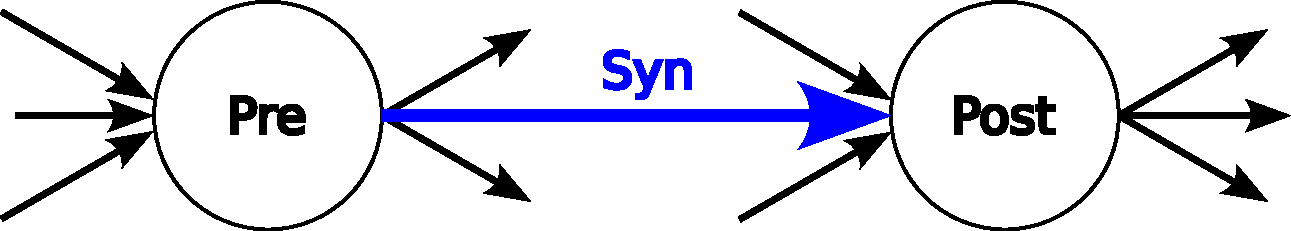
\includegraphics[width=0.9\columnwidth]{Figures/pre_post_neuron.pdf}
    \caption{Basic Synaptic Connection}
    \label{fig:pre_post_neuron}
\end{figure}
If a neuron receives several spikes within a sufficiently small temporal window (dependent on the neuron's characteristics), the potentials triggered by them will be summed together. Depending on whether the incoming spikes triggering these potentials are excitatory or inhibitory, the resulting potentials are called excitatory or inhibitory post-synaptic potentials (EPSP/IPSP). If the membrane potential subsequently reaches a certain threshold (called \textit{action potential}), it will rapidly decrease its membrane potential by unloading it in the form of a spike. Over time the membrane potential deteriorates on itself however, so when the same number of excitatory spikes arrives at the neuron over a longer period of time, or when they are mixed with inhibitory spikes, they might not be able to trigger the action potential. The underlying dynamics of the handling of incoming spikes are referred to as \textit{synaptic integration}, which is why neuron models that are based on this mechanic to determine when to trigger a neuron to fire are called integrate-and-fire (IAF or I\&F) models.\\
The descriptions above are not accurate to the actual proceedings in brain cells and neglect many important biological structural components like dendrites, somata, and axons, to include them in the description of the synapse or neuron. This abstraction is made among other reasons to simplify these models to make them computationally less expensive. 

\section{Synaptic Plasticity}
With the basic structural backgrounds of spiking neural networks out of the way, a synaptic characteristic of critical importance to biological neural networks and the main research object of this thesis is still remaining. The talk is about \textit{synaptic plasticity},  which is generally assumed to be the substrate for learning and memory in cortical circuits \parencite{morrison_diesmann_gerstner_2008}.\\
Plasticity is a property of synapses that makes them form, strengthen, and degrade - for the most part - based on the spiking behavior of the neurons they connect. Due to plasticity being a massively complex mechanic of biological neural networks, that is composed of many different drivers for synaptic weight change, there is no easy way to describe it, which is why over the years, researchers came up with various rules and mathematical models to describe it. In the following two different kinds of plasticity will be briefly introduced.

\subsection{Short-Term Plasticity (STP)} \label{ssec:short_term_plasticity}
As the name already suggests, short-term plasticity operates on rather short timescales in the order of 100s of milliseconds. It can facilitate (STF) or depress (STD) synaptic connections based on the recent spiking history of a presynaptic neuron. A qualitative illustration of STP can be seen in Figure \ref{fig:stp_example} \parencite{morrison_diesmann_gerstner_2008}, where $\text{t}^\text{f}$ denotes an example spike at time $t$ and $x(t)$ is the corresponding postsynaptic membrane potential resulting from the spike.\\
Generally, when a neuron receives a spike, its membrane potential also spikes up and then slowly decreases again as visualized by $x(t)$. Without STP, spikes with very short interspike intervals (ISIs) would continuously increase this way. But based on whether the synapse is depressing or facilitating this behavior is changed. To be more precise, STP in depressing synapses causes the increase in membrane potential to stagnate when many spikes come in with short ISIs by amplifying the decrease after an incoming spike for a short window of time. STP on facilitating synapses on the other hand causes the postsynaptic potential to decrease slower the smaller the ISIs of the incoming spikes are.

\begin{figure}[htbp]
    \centering
    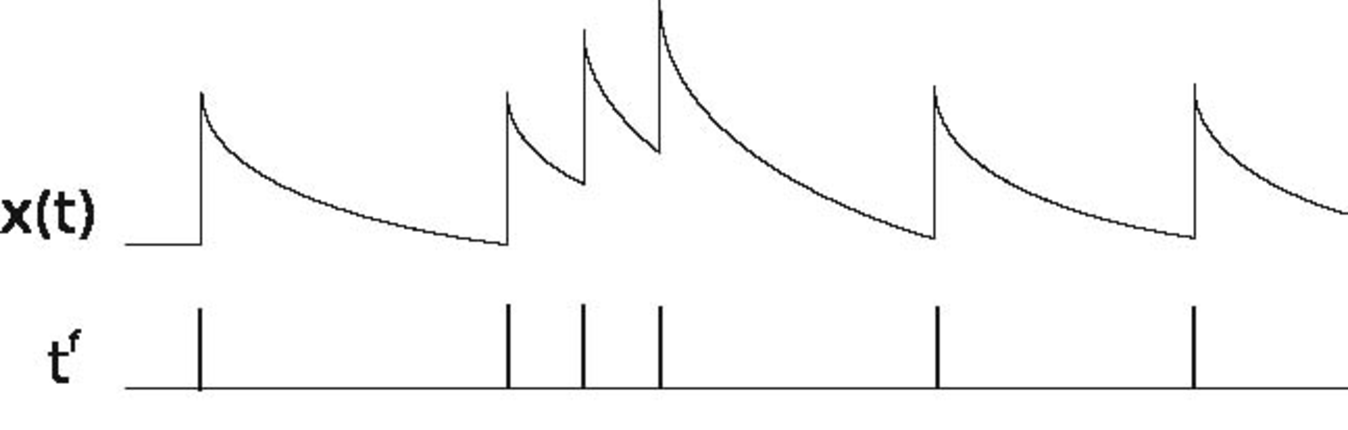
\includegraphics[width=0.9\columnwidth]{Figures/stp_example.pdf}
    \caption{STP Example \parencite{morrison_diesmann_gerstner_2008}}
    \label{fig:stp_example}
\end{figure}


\subsection{Spike-Timing-Dependent Plasticity (STDP)} \label{ssec:spike_timing_dependent_plasticity}
Spike-timing-dependent plasticity is a form of structural plasticity that, unlike STP, allows long-term consolidation of learned behavior by adjusting the efficacy of the synapse based on the learned correlation of firing behavior. This can be better described by Hebb's postulate, an early rule for synaptic plasticity that applies well to STDP:
\begin{displayquote}
\textit{When an axon of cell A is near enough to excite a cell B and repeatedly or persistently takes part in firing it, some growth process or metabolic change takes place in one or both cells such that A’s efficiency, as one of the cells firing B, is increased.}
\end{displayquote}

\begin{wrapfigure}{R}{0.5\textwidth}
    \begin{center}
        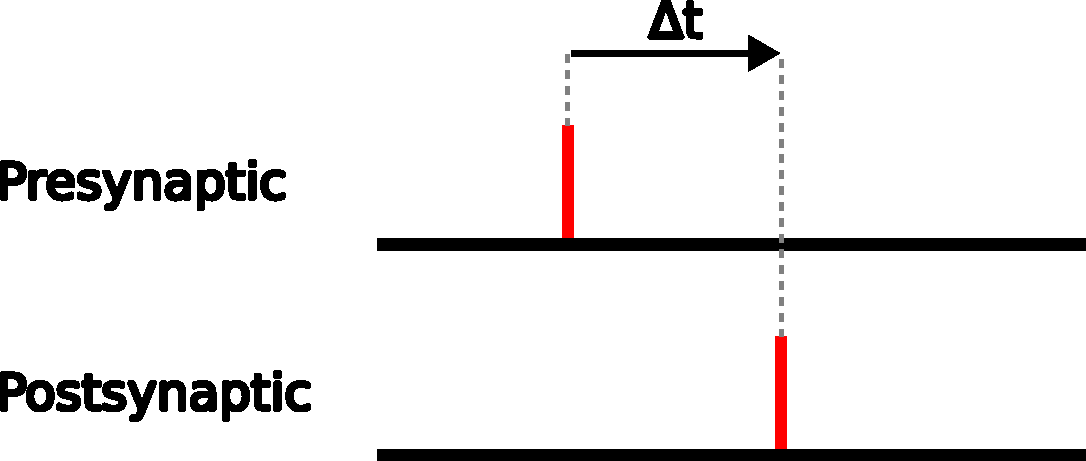
\includegraphics[width=0.48\textwidth]{Figures/pre_post_spikes.pdf}
    \end{center}
\caption{Pre- and Postsynaptic Spikes}
\label{fig:pre_post_spikes}
\end{wrapfigure}
Thus, when a postsynaptic neuron receives a spiking input from a presynaptic source shortly before firing as illustrated in Figure \ref{fig:pre_post_spikes}, the source is more likely to have a causal effect on the postsynaptic neuron, which justifies the facilitation of the connecting synapse. On the other side, if the spiking behavior of the postsynaptic neuron and the source are independent, the connection is degraded. This is a form of correlation-based unsupervised learning, but due to the popularity of Hebb's postulate, it is also referred to as Hebbian learning \parencite{morrison_diesmann_gerstner_2008}.

% Chapter Template

\chapter{Original Work} % Main chapter title

\label{Chapter3} % Change X to a consecutive number; for referencing this chapter elsewhere, use \ref{ChapterX}

\section{Outline}
The original work of \parencite{klampfl_maass_2013} that is replicated in this paper is based on the \textit{liquid computing model}. This computing paradigm is loosely inspired by biological brains and offers a way of implementing Spiking Neural Networks (SNNs). It consists of a collection of nodes (that resemble neurons) that can send and receive temporal signals (also called spikes) to and from other nodes via dedicated connections (which resemble synapses). These connections - just like the nodes - can have various other properties, such as delay or weight that influence how spikes are transmitted over the network of nodes. Additionally, neurons also possess a spatial coordinate that is necessary for having distance-dependent connection probabilities just like in the brain.\\
The conventional liquid computing model abstracts a fair amount of detail however, when compared to real cortical circuits. This includes a major structural trait inherent to the brain, that is assumed to enable long-term memory by forming stereotypical assemblies of neurons: synaptic plasticity. In the original paper, two forms of plasticity are used: short-term plasticity (STP) and spike-time dependent plasticity (STDP).\\
This chapter will first describe the initial structural setup of the network from the original implementation in Section \ref{sec:basic_network_structure} and then lay out how the generation and distribution of outside input is handled in Section \ref{sec:input_generation}. Finally, the dynamic properties that give the model its actual capabilities are discussed in Section \ref{sec:dynamic_network_behaviour}.

\section{Basic Network Structure} \label{sec:basic_network_structure} % including lateral inhibition
\begin{figure}[htbp]
  \centering
  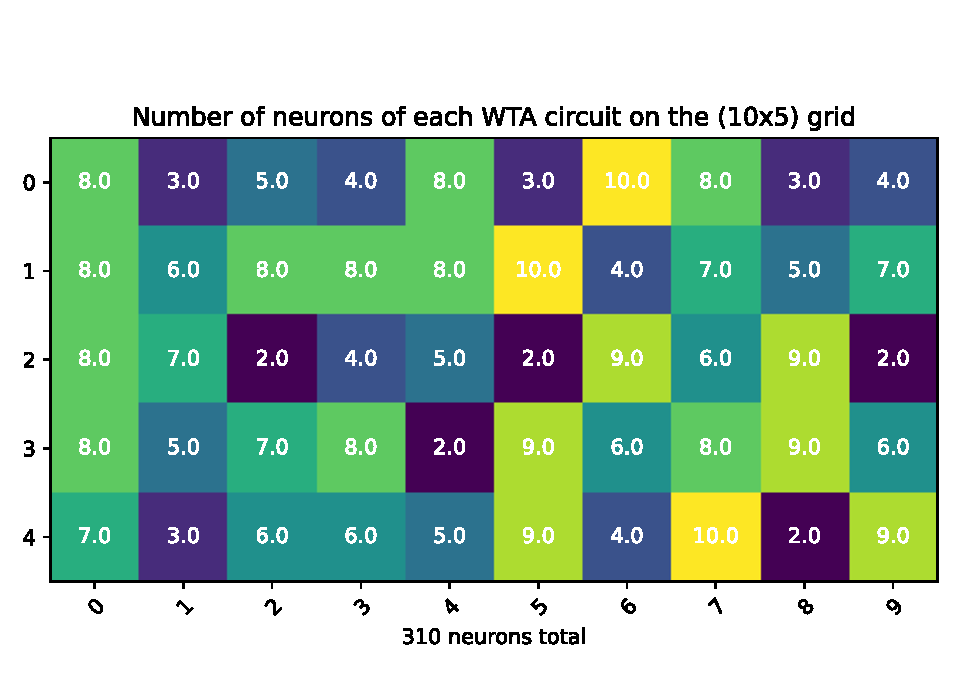
\includegraphics[width=0.9\columnwidth]{Figures/circuit_grid2D.pdf}
  \caption{Visualization of a random $10\times 5$ WTA circuit grid with $k_{min}=2, k_{max}=10$}
  \label{fig:circuit_grid}
\end{figure}
The basic setup of the liquid computing model employs a 2D grid of so-called Winner-Take-All (WTA) circuits, usually set to a size of $10\times 5$ as in the example grid in Figure \ref{fig:circuit_grid}. The 2D grid is utilized to assign spatial coordinates to each WTA, for the purpose of constructing inter-circuit connections with distance-dependent probability. The reason for this is that it has been found that in the brain, the probability that two neurons are synaptically connected decreases as their spatial distance increases. To describe this structural property mathematically, there exist multiple different rules including the following chosen for the original implementation:
\begin{equation}
    p(d)=\lambda e^{-\lambda d} \label{eqn:distance_dependent_probability}
\end{equation}
where $d$ is the euclidean distance between two WTA circuits and $\lambda$ is a generic setting parameter for adapting the connectivity rule to work well with the given grid size. In the original implementation $\lambda=0.088$.\\
The WTA circuits themselves are each composed of neurons $z_1, \dots, z_K$, where the integer $K$ is uniformly drawn at random from a range $[k_{\min}, k_{\max}]$. All neurons $z_1, \dots, z_K$ in the same WTA are not laterally connected and are subject to a mechanic called lateral inhibition. This is illustrated in Figure \ref{fig:wta_circuit}. Lateral inhibition causes that when one neuron in the WTA circuit fires, all other neurons in the same circuit experience inhibition, i.e. are discouraged from also firing. The biologically most accurate solution for implementing it would be to introduce inhibitory neurons that receive input from the entire WTA and output inhibitory spikes to the same circuit (as seen in Fig. \ref{fig:wta_circuit}).\\
In \parencite{klampfl_maass_2013} this is however said to be realized in a different way, by adjusting the firing rate of each neuron $k$ according to the summed firing rate of the WTA like this:
\begin{equation}
    r_k(t)=R_{\max}\cdot \frac{e^{u_k(t)}}{\sum_{j=1}^{K} e^{u_j(t)}}
    \label{eqn:firing_rate_paper}
\end{equation}
$R_{\max}$ is a fixed value that defines the maximum firing rate and is usually set to \SI{100}{\hertz}. $u_k(t)$ on the other hand stands for the current membrane potential of neuron $z_k$ at time $t$ and will be explained in more detail in Section \ref{sec:dynamic_network_behaviour}.
This realization of lateral inhibition bypasses the use of dedicated inhibitory neurons for lateral inhibition but is also responsible for normalizing the firing rate of the combined WTA circuit to $R_{\max}$, even when no external inputs are present. In principle, this is an unwanted side-effect, but according to \parencite{klampfl_maass_2013}, this is insignificant to the results of their study. Replacing this mode of lateral inhibition might be interesting for future work with the model from their paper.\\

\begin{figure}[htbp]
  \centering
  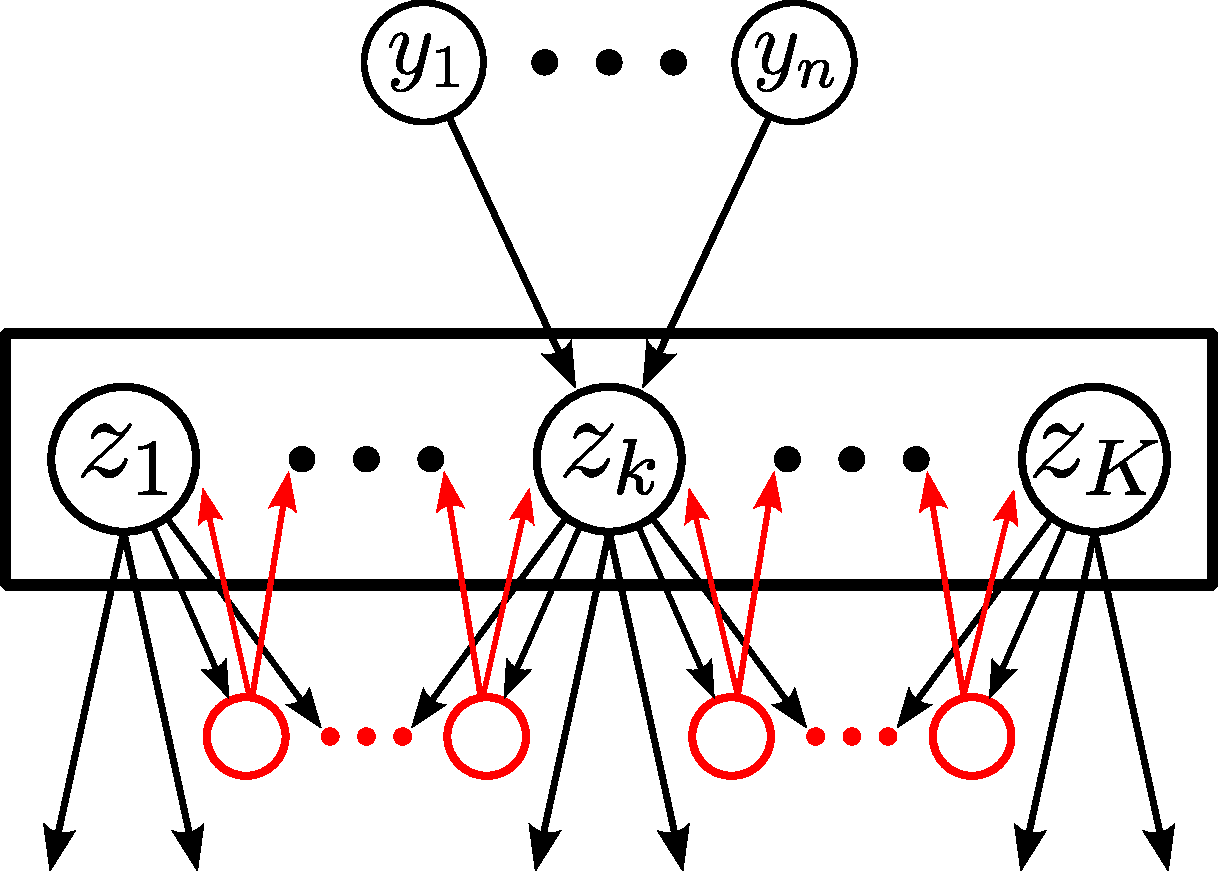
\includegraphics[width=0.8\columnwidth]{Figures/wta_circuit.pdf}
  \caption{WTA circuit with lateral inhibition}
  \label{fig:wta_circuit}
\end{figure}

\section{Running the Network} \label{sec:running_the_network}
The original model offers two different functions of running the network and producing readouts: \texttt{test()} and \texttt{simulate()}. The core difference is that during testing the network is not trained, i.e. the usual dynamic behavior resulting from STDP is disabled so that weights are not updated while running. STP is always enabled, while the use of variance tracking (described in Section \ref{sec:variance_tracking}) is optional but seems to be a requirement for learning with STDP, based on trials conducted with the original code. These findings are further discussed in Chapter \ref{Chapter5}.\\
Apart from the enabling of STDP, \texttt{test()} and \texttt{simulate()} are similar and share the same basic functionality. The network is run by progressing it step by step, where one step usually represents a time span of \SI{1}{\ms} (depending on the value of \texttt{dt}), after which the network states are updated according to the rules specified in Section \ref{sec:dynamic_network_behaviour}.

\section{Input Generation} \label{sec:input_generation}
To train the network properly for different tasks, the generation of input is key. In its simplest form, this is implemented as the presentation of recurrent pattern inputs, as illustrated in Figure \ref{fig:input_generator}. More complex sequences can also be generated based on this, but this will be briefly discussed in Chapter \ref{Chapter4} as it is not crucial for the tests performed in this thesis. The patterns here (represented by the grey boxes) consist of a number of input spike trains, where each input source gets its own Poisson spike train generated. Poisson generation is essentially realized by randomly sampling a list of values from an exponential distribution
\begin{equation}
    f(x;\frac{1}{\beta})=\frac{1}{\beta}\exp{\left(-\frac{x}{\beta}\right)},
    \label{eqn:exponential_distribution}
\end{equation} 
where $\beta$ corresponds to the firing rate in \SI{}{\hertz} of each spike train in that pattern. This list is then cumulatively summed, i.e. the list of values $v_1, \dots, v_k$ is updated as follows: $v_n\prime=\sum_{i=0}^{n-1} v_i$ to obtain an ascending list $v_1\prime, \dots, v_k\prime$ of spike times with interspike intervals (ISIs) drawn from Equation \ref{eqn:exponential_distribution}. This pattern generation has to be done once for every pattern before the network is run with pattern inputs.\\
These pattern inputs are however not the only kind of input that the network neurons receive. Unless disabled, they also receive random noise of frequency \texttt{rNoise} [\SI{}{\hertz}], which is constantly overlaid. The resulting two different types of total input can therefore be distinguished into noise and pattern phases of duration \texttt{tNoise} and \texttt{tPattern} respectively, where \texttt{tNoise} is uniformly drawn at random from the pre-specified interval \texttt{tNoiseRange}.\\
As already explained in Section \ref{sec:running_the_network}, the simulation is progressed stepwise. The same goes for the presentation of input. During each simulation step a function \texttt{generate(t)} is run on the input generator object, where \texttt{t} is the current time step of the simulation, displayed conceptually as the red dotted line in Fig. \ref{fig:input_generator}. For most decisions, the input generator works with the current time relative to the beginning of the last pattern: \texttt{tp=t-last\_pattern\_start}. A typical cycle for the simple example would for example be: present current pattern while \texttt{tp}$\leq$\texttt{tPattern}. As soon as \texttt{time\_to\_draw=0}, the \texttt{last\_pat\-tern\_start} is set to \texttt{t} and the pattern gets presented again for \texttt{tPattern}.

\begin{figure}[htbp]
  \centering
  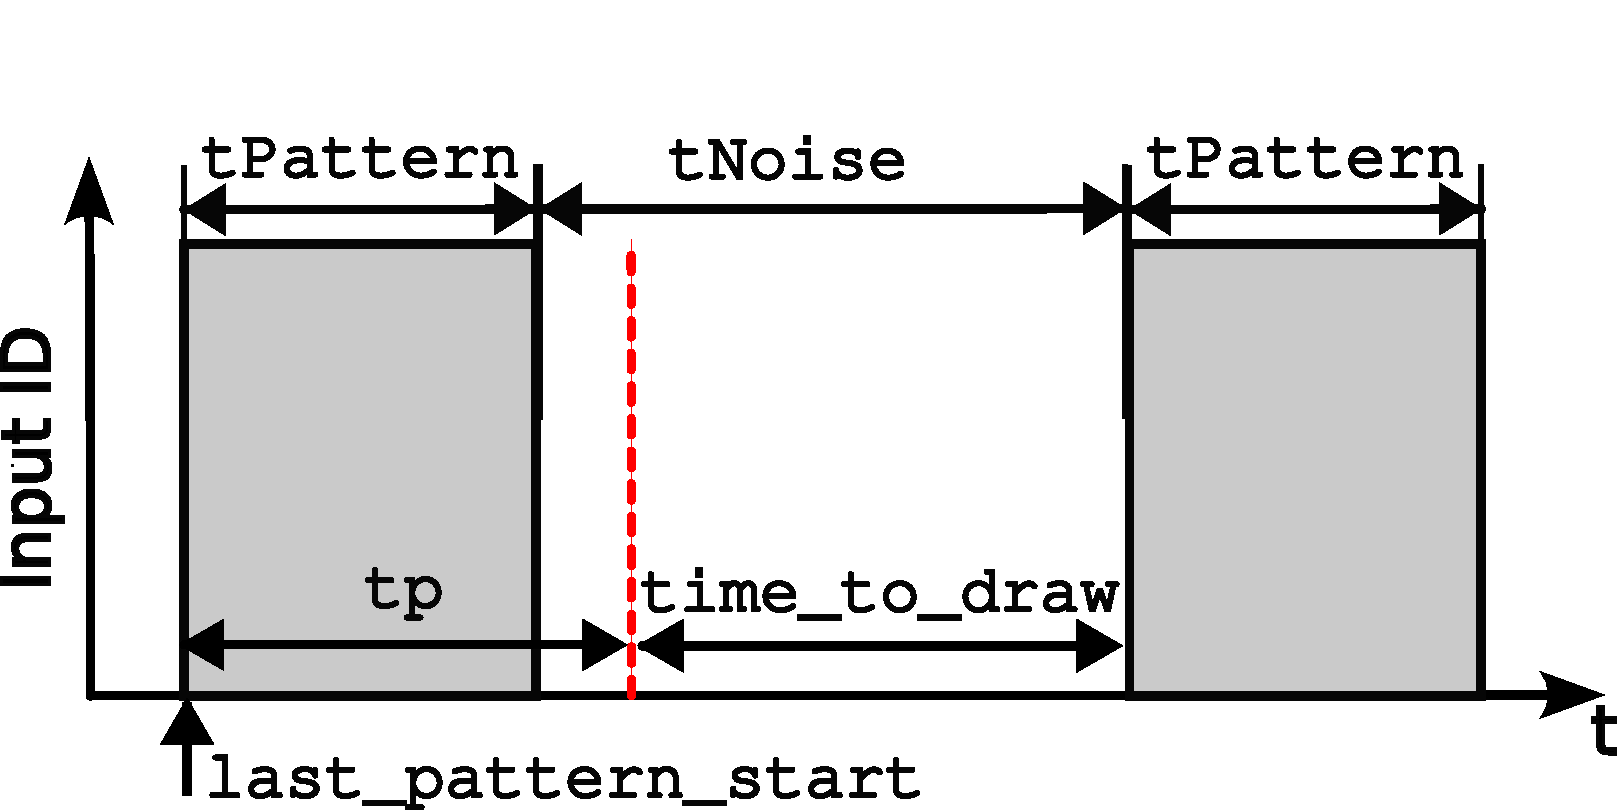
\includegraphics[width=0.9\columnwidth]{Figures/input_generator.pdf}
  \caption{Pattern Input Generation}
  \label{fig:input_generator}
\end{figure}

% Snippets
% Each input is connected to all neurons
% For more elaborate tasks pattern\_sequences are the way to go

\section{Dynamic Network Behaviour} \label{sec:dynamic_network_behaviour}
Now that the foundations of the network have been explained, it is time to dive into the actual dynamics which implement the models of plasticity and with them the ability of sequential learning. The cornerstone for neuron dynamics is the rule for determining the current membrane potential $u_k(t)$ of neuron $z_k$ (excluding the effect of lateral inhibition, which is added in \ref{eqn:firing_rate_paper}):
\begin{equation}
    u_k(t)=\sum_{i=1}^{n} w_{ki}y_i(t) + w_{k0}.
    \label{eqn:membrane_potential}
\end{equation}
Here $w_{ki}$ is the synaptic weight of an input synapse to neuron $z_k$ from pre-synaptic neuron $y_i$, and $w_{k0}$ is a bias parameter of the $k$-th neuron. This parameter has, however, no effect on the membrane potential in the implementation since it is initially set to zero and never updated. It is therefore ignored for the rest of this thesis. Finally, $y_i(t)$ fittingly denotes the current value for the excitatory postsynaptic potential (EPSP) of presynaptic neuron $y_i$. This potential is modelled as an $\alpha$-shaped kernel with rise time constant $\tau_{\text{rise}}=\SI{2}{ms}$ and decay time constant $\tau_{\text{decay}}=\SI{20}{ms}$ as follows:
\begin{equation}
    y_i(t)= \underset{t_p}{\sum} \exp\left(-\frac{t-t_p}{\tau_{\text{decay}}}\right) - exp\left(-\frac{t-t_p}{\tau_{\text{rise}}}\right)
    \label{eqn:epsp}
\end{equation}
\begin{equation*}
    \left(= \underbrace{\underset{t_p}{\sum} \exp\left(-\frac{t-t_p}{\tau_{\text{decay}}}\right)}_{\approx\texttt{epsp}} - \underbrace{\underset{t_p}{\sum} exp\left(-\frac{t-t_p}{\tau_{\text{rise}}}\right)}_{\approx\texttt{epsp2}}\right)
\end{equation*}
where $t_p$ is the set of presynaptic spike times at time $t$. This EPSP is also implemented somewhat differently from the mathematical description in Equation \ref{eqn:epsp}, which is why it was decided here to add the conversed equation for $y_i(t)$ in braces. As pointed out there, the parts of the conversed equation are realized in the code by the two variables \texttt{epsp} and \texttt{epsp2}, standing for the current EPSP values when solely considering the EPSP resulting from decay and rise respectively. While they serve the same purpose as their representations in the equation they work differently. Essentially, each of these ESPS variables decrease over time by 
\begin{equation}
    \texttt{epsp}_t=\texttt{esps}_{t-1} \left(1-\frac{\texttt{dt}}{\texttt{tau}} \right)
    \label{eqn:epsp_update}
\end{equation}
with \texttt{dt}=0.001 the simulation time step in seconds and \texttt{tau} the time constant of the \texttt{epsp} (either $\tau_{\text{rise}}$ or $\tau_{\text{decay}}$). With the decrease in EPSP for the rise and decay phases explained this still leaves the EPSP-increasing behavior undescribed. Although this is not directly mentioned in \parencite{klampfl_maass_2013}, this is in fact done by the STP mechanic described in the paper, which is why this will be further discussed in Section \ref{ssec:stp}. All that will be said about this here is that in the case of an incoming spike, the EPSP for both \texttt{epsp} and \texttt{epsp2} will be updated by $\Delta \texttt{epsp}=u\cdot R$ in addition to the EPSP decreasing behavior with $u,R\in[0,1]$ being dynamic variables that are defined in Equation \ref{eqn:stp}. 

%In the original implementation code most attributes that need to be defined per neuron or synapse (like weight and membrane potential) are handled using large arrays

\subsection{STP} \label{ssec:stp}
STP is a form of plasticity that changes the efficacy of a synapse on the scale of a few hundred to thousands of milliseconds \parencite{stevens_wang_1995}. It can be further categorized into Short-Term Facilitation (STF) and Short-Term Depression (STD) and generally causes the strength of an incoming spike to be determined also by the previous recently incoming spikes, instead of simply the synaptic weight.\\
As is clear from Equations \ref{eqn:membrane_potential} and \ref{eqn:firing_rate_paper}, there are two options in the current model to manipulate the dynamics of firing rates: using synaptic weights or EPSPs. Because STP only temporarily changes the synaptic efficacy, it makes more sense to implement it by manipulating EPSPs, which is what happens in \parencite{klampfl_maass_2013}. They determine the amplitude $A_k$ of the $k$-th input spike as follows:
\begin{equation}
\begin{aligned}
    A_k &= w_k \cdot \overbrace{u_k \cdot R_k}^{=\Delta\texttt{epsp}}\\
    u_k &= U + u_{k-1}(1-U)\exp(-\Delta_{k-1}/F)\\
    R_k &= 1 + (R_{k-1} - u_{k-1}R_{k-1}-1)\exp(-\Delta_{k-1}/D)\\
\end{aligned}
\label{eqn:stp}
\end{equation}
It is important to define the notion of "amplitude" more clearly here. Amplitude in this context refers to a combined metric of synaptic weight and EPSP associated with each given spike. The EPSP that is calculated by $u_k\cdot R_k$ was already introduced when describing the EPSP in Equation \ref{eqn:epsp} and is responsible for the EPSP increase on spike input.\\
The interspike intervals of the entire spike train up to the $k$-th spike are given by $\Delta_1, \Delta_2, \dots, \Delta_{k-1}$, while $D$ and $F$ are STD- and STF-related time parameters. $U$, $D$ and $F$ all have in common that they are set randomly for each synapse from Gaussian distributions $\mathcal{N}(\mu, \sigma^2)$ with $\sigma=0.5\mu$ and $\mu_U=0.5$, $\mu_D=0.11$, $\mu_F=0.005$. In the implementation the additional constraints $U\geq 0$, $D,F\geq \texttt{dt}$ are added to ensure that the amplitude does not take on unintended values.\\
% [describe the effect of this plasticity rule]
Klampfl and Maass stated they adopted this short-term plasticity model from \parencite{markram_wang_tsodyks_1998}. However, on comparison, it is noticeable a detail was altered when doing so. Instead of the definition of $R_k$ from Equation \ref{eqn:stp}, the following definition  would conform with their cited model:
\begin{equation*}
    R_k = 1 + (R_{k_1} - \mathbf{u_{k}}R_{k-1}-1)\exp(-\Delta_{k-1}/D)
\end{equation*}
with $u_k$ instead of $u_{k-1}$. It is unclear if this detail has any significant effect and if it was an intentional decision that was simply not explained by Klampfl and Maass, but it is worth mentioning and should be considered when using their model for future work.\\
Another mistake of the computational kind was also found in the original implementation. Usually, only recurrent connections should be subject to STP, but due to an error in the calculation of $R_k$, STP was partially applied to input connections as well.


\subsection{STDP} \label{ssec:stdp}

STDP, unlike STP, is a long-term plasticity that is based on temporal differences between pre- and post-spikes. More precisely, this means that whenever a postsynaptic neuron $z$ emits a spike at time $t_{post}$ and receives an incoming spike from presynaptic neuron $y$ at time $t_{pre}$, then the weight of the connecting synapse is increased if $t_{pre}< t_{post}$ and decreased if $t_{pre}\geq t_{post}$. There are many different rules that model STDP, but Klampfl and Maass stated they wanted to implement it using the following weight update rule:
\begin{equation}
    \Delta w_{ki}=y_i(t) \cdot c \cdot e^{-w_{ki}} - 1 = \frac{c\cdot y_i(t)-e^{w_{ki}}}{e^{w_{ki}}},
    \label{eqn:stdp_paper}
\end{equation}
where $w_{ki}$ denotes the weight of the synapse input to neuron $z_k$ from pre-synaptic neuron $y_i$. This weight update should be performed every time neuron $z_k$ fires. Furthermore, $y_i(t)$ denotes the current value of the EPSP at presynaptic neuron $y_i$ as formulated in Equation \ref{eqn:epsp} and $c$ is a scaling parameter used to keep the synaptic weights in a positive range. This parameter is comprised of the learning rate $\eta^*=0.05$ and an offset of $5$ like this: $c=0.05 \cdot \exp(5)=7.42$.\\
Obviously, this STDP model does not make use of $t_{pre}$ and $t_{post}$ directly, which is somewhat unusual. It rather exploits the fact that the EPSP $y_i(t)$ of the presynaptic neuron should be high if it has recently spiked, and low if it has not spiked in the recent past. To better visualize STDP a common way is to plot an STDP window. STDP windows can be created practically by setting a fixed spike time for the post-spike of a neuron and confronting it with varying pre-spike times. For each pre-/post-spike combination, the resulting weight change is plotted. For the STDP rule from Equation 5 of \parencite{klampfl_maass_2013} this produces the STDP window in Figure \ref{fig:stdp_window}. 
As illustrated there, the weight is reduced by a constant of $-1$ every time a pre-spike arrives earlier than the post-spike is emitted and is only ever increased if the pre-spike comes in later, but only for a brief period of time.\\
\begin{figure}[htbp]
    \centering
    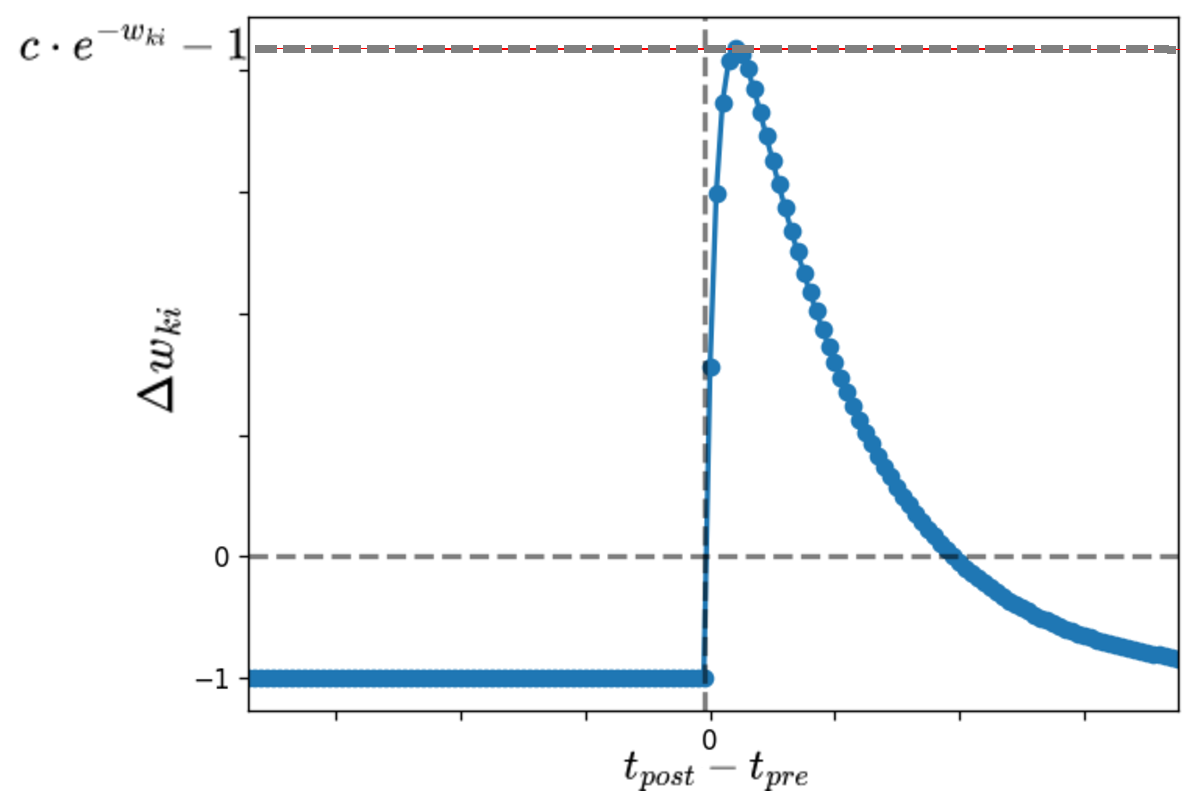
\includegraphics[width=0.7\columnwidth]{Figures/stdp_window.pdf}
    \caption{STDP window}
    \label{fig:stdp_window}
\end{figure}
\\ \ \\ % [TODO: STDP window from paper]
% [maybe TODO: explain STDP window above]
It is also claimed in the original paper that the bias parameter from Equation \ref{eqn:membrane_potential} is updated by the following rule:
\begin{equation*}
    \Delta w_{k0} = 
    \begin{cases}
        c\cdot e^{-w_{k0}} -1 & \text{if neuron } z_k \text{ fires}\\
        -1 & \text{else}
    \end{cases}
\end{equation*}
However, this could not be found in the implementation code, which is why it will not be regarded for the replication. Apart from this, the actual implementation of $\Delta w_{ki}$ also seems to deviate slightly from Equation \ref{eqn:stdp_paper}:
\begin{equation}
    \Delta w_{ki} = \eta_{ki} \cdot \frac{y_i(t)-e^{w_{ki}}}{\max \{e^{w_{ki}}, \eta_{ki}\}}
    \label{eqn:stdp_real}
\end{equation}
The reason for this is that Klampfl and Maass decided to also adopt adaptive learning rates for synapses from \parencite{nessler_et_al_2013}. This is handled by the synapse-specific learning rate $\eta_{ki}$, which replaces the static parameter $c$.

\subsubsection{Variance Tracking} \label{sec:variance_tracking}
The integration of adaptive learning rates is done by a heuristic called variance tracking, described in \parencite{nessler_et_al_2013}. Its purpose is to facilitate the spontaneous reorganization of the learned models (encoded in the form of synaptic weights) in the event that the input distribution $p^*(\mathbf{y})$ changes. The input distribution $p^*(\mathbf{y})$ would for example change when a new different spike pattern would be presented to the network for learning.\\
This variance tracking is defined in Equation 71 of \parencite{nessler_et_al_2013}:
\begin{equation}
    \eta_{ki}^{new} = \frac{ \text{E}[w_{ki}^2] - \text{E}[w_{ki}]^2 }{ e^{-\text{E}[w_{ki}]} + 1 } 
    = \frac{ \text{Var}(w_{ki}) }{ e^{-\text{E}[w_{ki}]} + 1 },
    \label{eqn:variance_tracking}
\end{equation}
which is used to calculate $\eta_{ki}=\eta^*\cdot \eta_{ki}^{new}$. In the following let $S_{ki}:=\text{E}[w_{ki}]$ and $Q_{ki}:=\text{E}[w_{ki}^2]$, as these variables are used in the original implementation. The way their values are determined there is by summing over the presynaptic spike times $t_p$ of their associated synapse up to the current point in time:
\begin{equation}
\begin{aligned}
    S_{ki}^{(t)} &= \sum_{t_p}^t \eta_{ki}^{(t_p)} \cdot (w_{ki}^{(t_p)}-S_{ki}^{(t_p)})\\
    Q_{ki}^{(t)} &= \sum_{t_p}^t \eta_{ki}^{(t_p)} \cdot (w_{ki}^2 {}^{(t_p)}-Q_{ki}^{(t_p)})\\
    \text{with } S^{(0)}&=0 \text{ and } Q^{(0)}=1
\end{aligned}
\label{eqn:variance_tracking_2}
\end{equation}

\section{Summary of Complications} \label{sec:summary_complications_original}
While working on this thesis, several major obstacles were encountered. Those specific to the paper and the associated code base are briefly summarized in this section for better outlining of difficult problems to avoid future issues.
\begin{itemize}
    \item The rates described in the paper differ from the implementation. This is further discussed in Section \ref{sec:input_generation}.
    \item Despite what the paper states about neurons being individually connected with probability $p(d)$, in the code only entire WTAs are connected to each other with all-to-all connections between their respective sets of neurons.
    \item As discussed in Section \ref{ssec:stdp}, the actual implementation of STDP differed clearly from the description in the paper.
    \item There was also an implementation error in the STP, where STP was partially applied to input synapses, which is not intended (mentioned in Section \ref{ssec:stp})
    \item The used STP rule in both paper and code is adopted incorrectly from the cited source in the paper (see Section \ref{ssec:stp})
\end{itemize}

% Snippets
% it was found that variance tracking is necessary

% list of important parameters that will be referenced e.g. when producing readouts for the network


% Chapter Template

\chapter{Implementation} % Main chapter title

\label{Chapter4} % Change X to a consecutive number; for referencing this chapter elsewhere, use \ref{ChapterX}

%----------------------------------------------------------------------------------------
%	SECTION 1
%----------------------------------------------------------------------------------------

\section{Overview}
Most of the implementation apart from the custom neuron and synapse models is written in Python 3.9. This offers the opportunity to create an object-oriented implementation, loosely inspired by the original work of \parencite{klampfl_maass_2013}. The fundamental object classes this project uses are:
\begin{itemize}
    \item \texttt{WTACircuit}: Serves as the basic component to organize sets of neurons that are supposed to form the same WTA circuit. (Section \ref{sec:wta_circuit_network})
    \item \texttt{Network}: The centerpiece of this project, implementing the grid composition of \texttt{WTACircuit} objects as well as the inter-network neuron connections. (Section \ref{sec:wta_circuit_network})
    \item \texttt{InputGenerator}: Responsible for the setup and tuning of pattern and noise input to the network during simulation. (Section \ref{sec:input_generation})
    \item \texttt{Recorder}: Manages the simulation of the associated \texttt{InputGenerator} and \texttt{Network} as well as the recording of Network properties like spiking input, network spike behavior, membrane potential, EPSP, and weight. Also responsible for plotting the recorded data. (Section \ref{sec:recording})
\end{itemize}
These object classes can be seen in Figure \ref{fig:implementation_concept_drawing} where their relation to each other, structure, and function is conceptually illustrated. It is important to point out, however, that the Python part of this project is only responsible for the organization, creation, and manipulation of NEST components like neurons, synapses, spike generators, and measurement devices. Most of the heavy lifting in the background required to operate and simulate these is outsourced to NEST. The source code for this thesis can be found in \parencite{michau_2022}.
\begin{figure}[htbp]
    \centering
    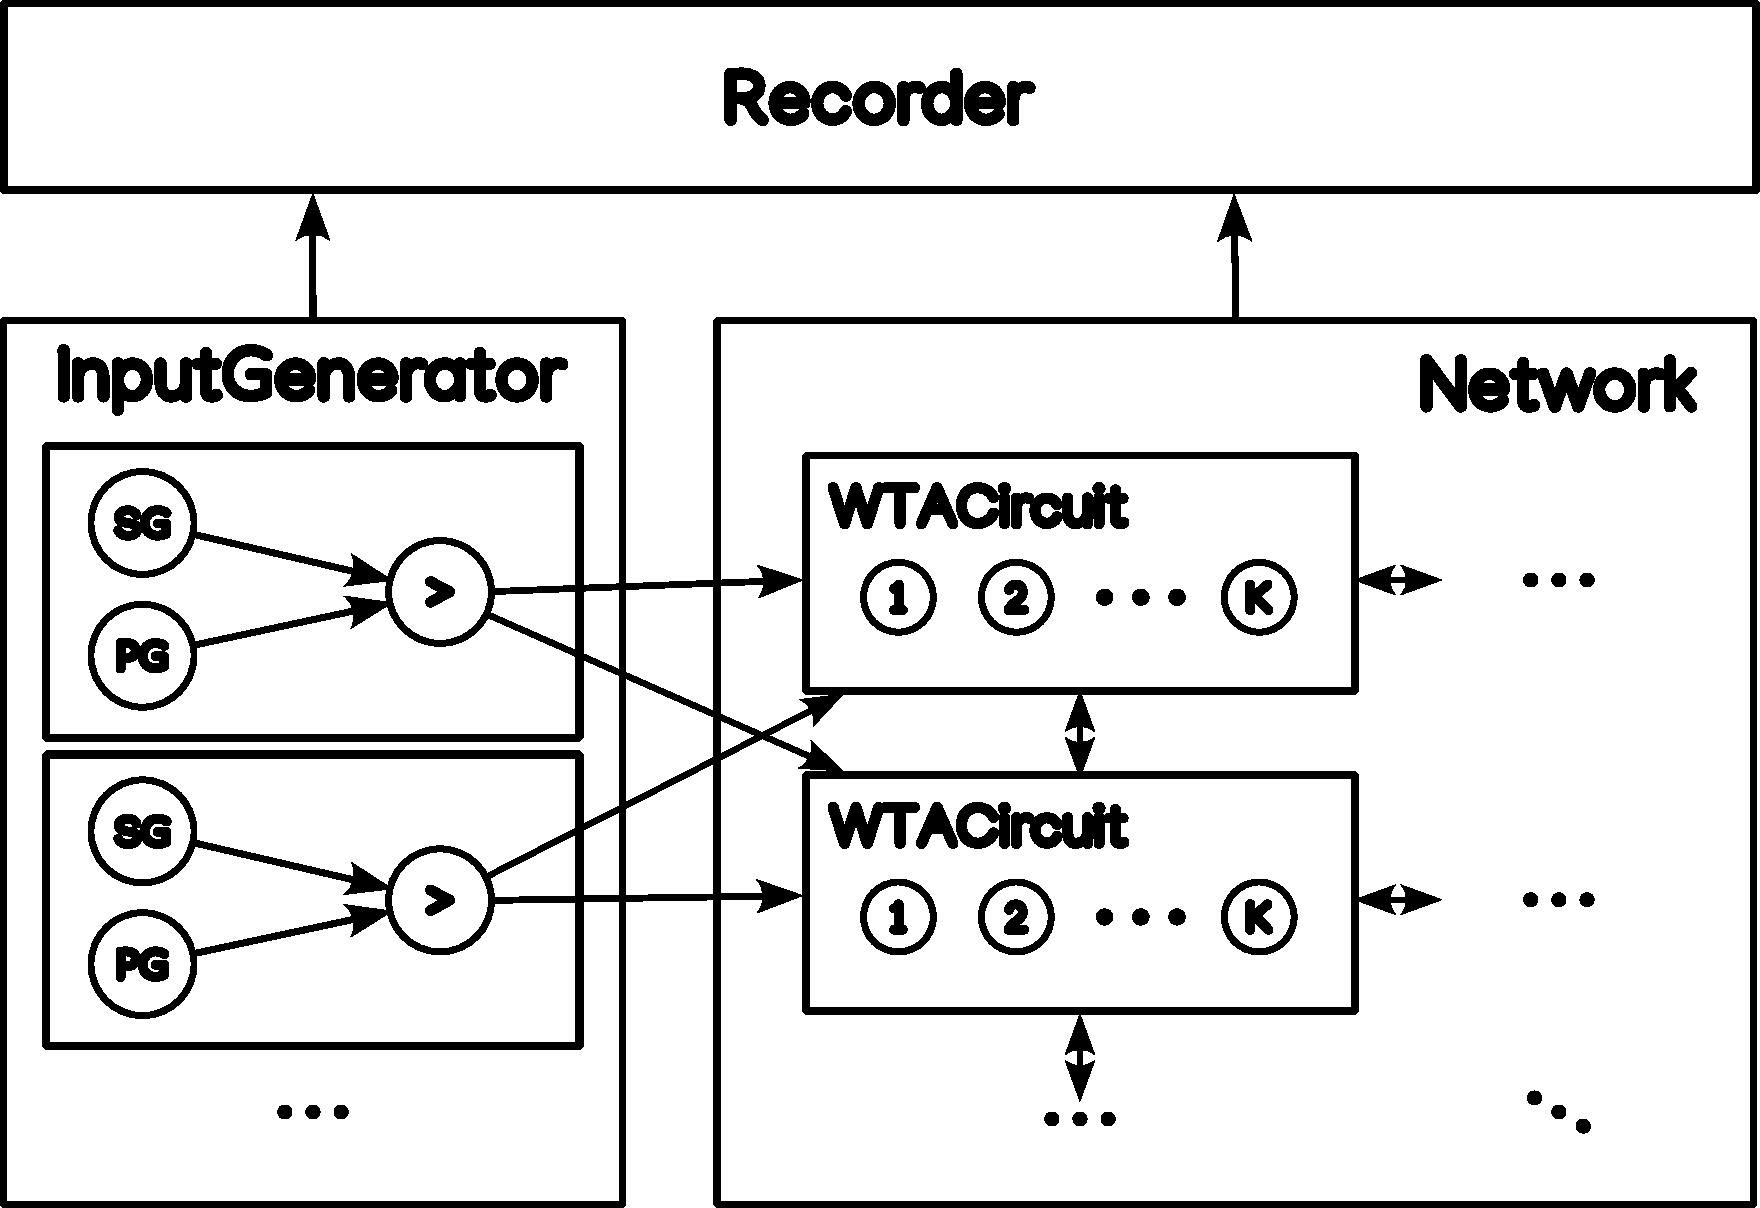
\includegraphics[width=\columnwidth]{Figures/implementation_conceptual.pdf}
    \caption{Conceptual Drawing of Implementation. Definition of terms: \textbf{SG} denotes 'Spikegenerator', \textbf{PG} denotes 'Poissongenerator' and \textbf{>} denotes 'Parrot neuron'.}
    \label{fig:implementation_concept_drawing}
\end{figure}

% name basic components and underlying design principle of the implementation
% describe basic functionality of nest/NESTML
\section{WTA Circuit Network} \label{sec:wta_circuit_network}
\subsection{Grid}
To model the distance-dependent connection probability described in Equation \ref{eqn:distance_dependent_probability} it is necessary to first assign each neuron in the network a spatial coordinate to determine the distance between different WTA circuits. While NEST provides the possibility to construct spatially structured spiking neural networks, together with a range of supporting functionality that is needed to replicate the model from \parencite{klampfl_maass_2013}, some details stand in the way of their use. First and foremost, the NEST spatially structured networks are designed to be biologically plausible, i.e. work in three dimensions, as do all their functionalities like e.g. functions to determine distances. Meanwhile, the \parencite{klampfl_maass_2013} model is rather implemented using a 2D grid where the coordinates are assigned on a per WTA basis, leading to multiple neurons having the same coordinates. As this would be difficult to implement in NEST, a simpler approach was pursued instead.\\
Instead of using NEST's spatially structured network functionality, a custom \texttt{WTACircuit} object (Figure \ref{fig:object_wta_circuit}) was introduced, featuring a 2D-coordinate \texttt{pos} indicating the position on the grid and a NodeCollection of size \texttt{k}:\\
\begin{figure}[htbp]
\centering
\begin{tikzpicture}
\begin{class}[text width=0.9\columnwidth]{WTACircuit}{0,0}
    \attribute{nc : \textbf{NodeCollection}}
    \attribute{pos : \textbf{tuple}}
    \attribute{k : \textbf{int}}
    \operation{\_\_init\_\_(nc: \textbf{NodeCollection}, pos: \textbf{tuple})}
    \operation{form\_WTA() $\rightarrow$ \textbf{NoneType}}
    \operation{get\_pos() $\rightarrow$ \textbf{tuple}}
    \operation{get\_x() $\rightarrow$ \textbf{int}}
    \operation{get\_y() $\rightarrow$ \textbf{int}}
    \operation{get\_node\_collection() $\rightarrow$ \textbf{NodeCollection}}
    \operation{get\_size() $\rightarrow$ \textbf{int}}
\end{class}
\end{tikzpicture}
\caption{\texttt{WTACircuit} Class Diagram} \label{fig:object_wta_circuit}
\end{figure}
\\
As can be seen from Figure \ref{fig:object_wta_circuit}, the \texttt{WTACircuit} object is initialized using a position tuple and a NodeCollection. This NodeCollection type is how NEST handles neurons of any kind that have been previously created. The initialization function \texttt{\_\_init\_\_()} also instantiates \texttt{k} with the size of the NodeCollection \texttt{nc} using \texttt{get\_size()} and most notably connects every neuron in \texttt{nc} to every other neuron via an InstantaneousRateConnection. These connections do not model any synapses and are in fact a makeshift solution that had to be manually implemented to the neuron model in C++ because they are necessary for the abstract implementation of lateral inhibition without dedicated inhibitory neurons as stated by \parencite{klampfl_maass_2013}, which is not provided by NEST or NESTML.
These InstantaneousRateConnections were originally developed in NEST for use in continuous rate models, where they would communicate rates. For this thesis, they were modified to enable the communication of membrane potentials within the WTA circuit. This is crucial for the calculation of the firing rate (Equation \ref{eqn:firing_rate_paper}) since each node has to calculate it on its own and is therefore dependent on the firing rates of its fellow neurons in the WTA.
\begin{figure}[htbp]
\centering
\begin{tikzpicture}
\begin{class}[text width=0.9\columnwidth]{Network}{0,0}
    \attribute{grid\_shape: \textbf{tuple}}
    \attribute{n: \textbf{int}}
    \attribute{m: \textbf{int}}
    \attribute{k\_min: \textbf{int}}
    \attribute{k\_max: \textbf{int}}
    \attribute{n\_inputs: \textbf{int}}
    \attribute{lam: \textbf{float}}
    \attribute{circuits: \textbf{list}}
    \attribute{save\_figures: \textbf{bool}}
    \attribute{show\_figures: \textbf{bool}}
    \operation{\_\_init\_\_(**kwds)}
    \operation{create\_grid() $\rightarrow$ \textbf{list}}
    \operation{form\_connections() $\rightarrow$ \textbf{NoneType}}
    \operation{get\_circuit\_grid() $\rightarrow$ \textbf{numpy.ndarray}}
    \operation{get\_node\_collections(slice\_min: \textbf{int}, slice\_max: \textbf{int}) $\rightarrow$ \textbf{NodeCollection}}
    \operation{get\_pos\_by\_id() $\rightarrow$ \textbf{tuple}}
    \operation{visualize\_circuits() $\rightarrow$ \textbf{NoneType}}
\end{class}
\end{tikzpicture}
\caption{\texttt{Network} Class Diagram} \label{fig:object_network}
\end{figure}
\\ \ \\
The \texttt{Network} object in turn uses the \texttt{WTACircuit}s to construct a grid of shape $\texttt{n}\times\texttt{m}$ with them, where each \texttt{WTACircuit} has its size \texttt{K} uniformly drawn at random from the interval $[\texttt{k\_min}, \texttt{k\_max}]$. After the creation of the WTA grid using \texttt{create\_grid()}, all neurons in the network regardless of WTA association are connected to each other with probability derived from the distance-dependent probability rule from Equation \ref{eqn:distance_dependent_probability}. Additionally, the formation of \textit{autapses} (self-recurrent connections from the neuron to itself) are disabled. Initially, the synaptic weights of these connections are set to $1$, but they can also be randomized just as in \parencite{klampfl_maass_2013} by assigning the weights to $-\log(x)$, where $x\in[0; 1]$ is a random number.

\section{Input Generation} \label{sec:input_generation}
\begin{wrapfigure}{r}{0.45\textwidth}
    \begin{center}
        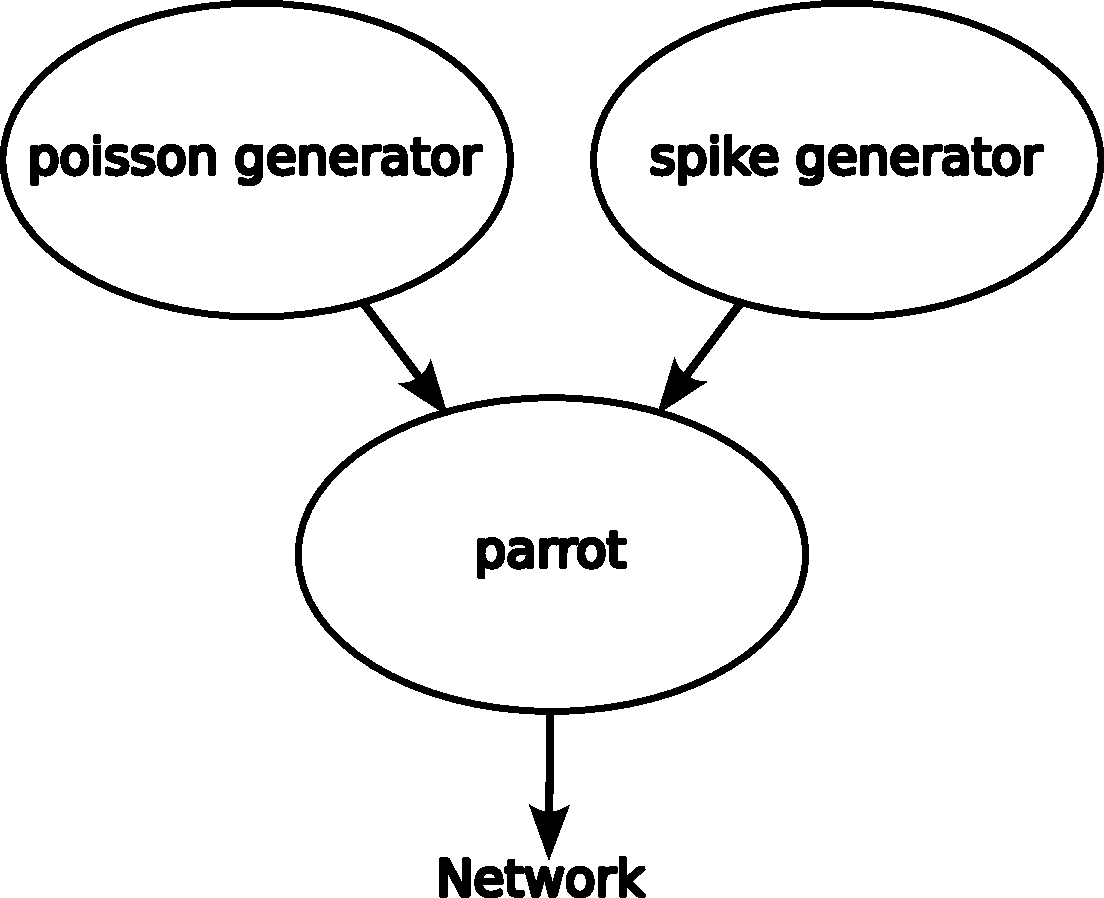
\includegraphics[width=0.4\columnwidth]{Figures/input_generator_structure.pdf}
    \end{center}
\caption{Single Input Assembly}
\label{fig:input_generator_structure}
\end{wrapfigure}
On the conceptual NEST level, each \texttt{InputGenerator} consists of \texttt{n} input assemblies as in Figure \ref{fig:input_generator_structure}. NESTs \textit{inhomogeneous\_poisson\_generator} is responsible for the creation of Poisson noise of specified rates for specified time intervals. The need for doing so is discussed later. 
Because a Poisson generator in NEST produces unique output for each neuron it is connected to - which is to be avoided to stay accurate to the original implementation - an additional \textit{parrot\_neuron} is interposed between the network and the Poisson generator. A parrot neuron in NEST just repeats the spikes it receives to all its connected targets, which effectively results in each network neuron receiving exactly the same noise input from the \textit{inhomogeneous\_poisson\_generator}.\\
The \textit{spike\_generator} handles the presentation of the pattern input as described in Chapter \ref{sec:input_generation}. Technically there is no need to connect it to a parrot, like the Poisson generator, but connecting it to the same parrot has the benefit that the input now enters the network over the same synapse. If the generator was connected to the network directly using its own synapse with plasticity, it is possible that the network might favor the pattern input over the noise by adjusting the synaptic weights, which would nullify the presence of noise in the first place. Also, this approach is more accurate to the original implementation.
\begin{figure}[htbp]
    \centering
    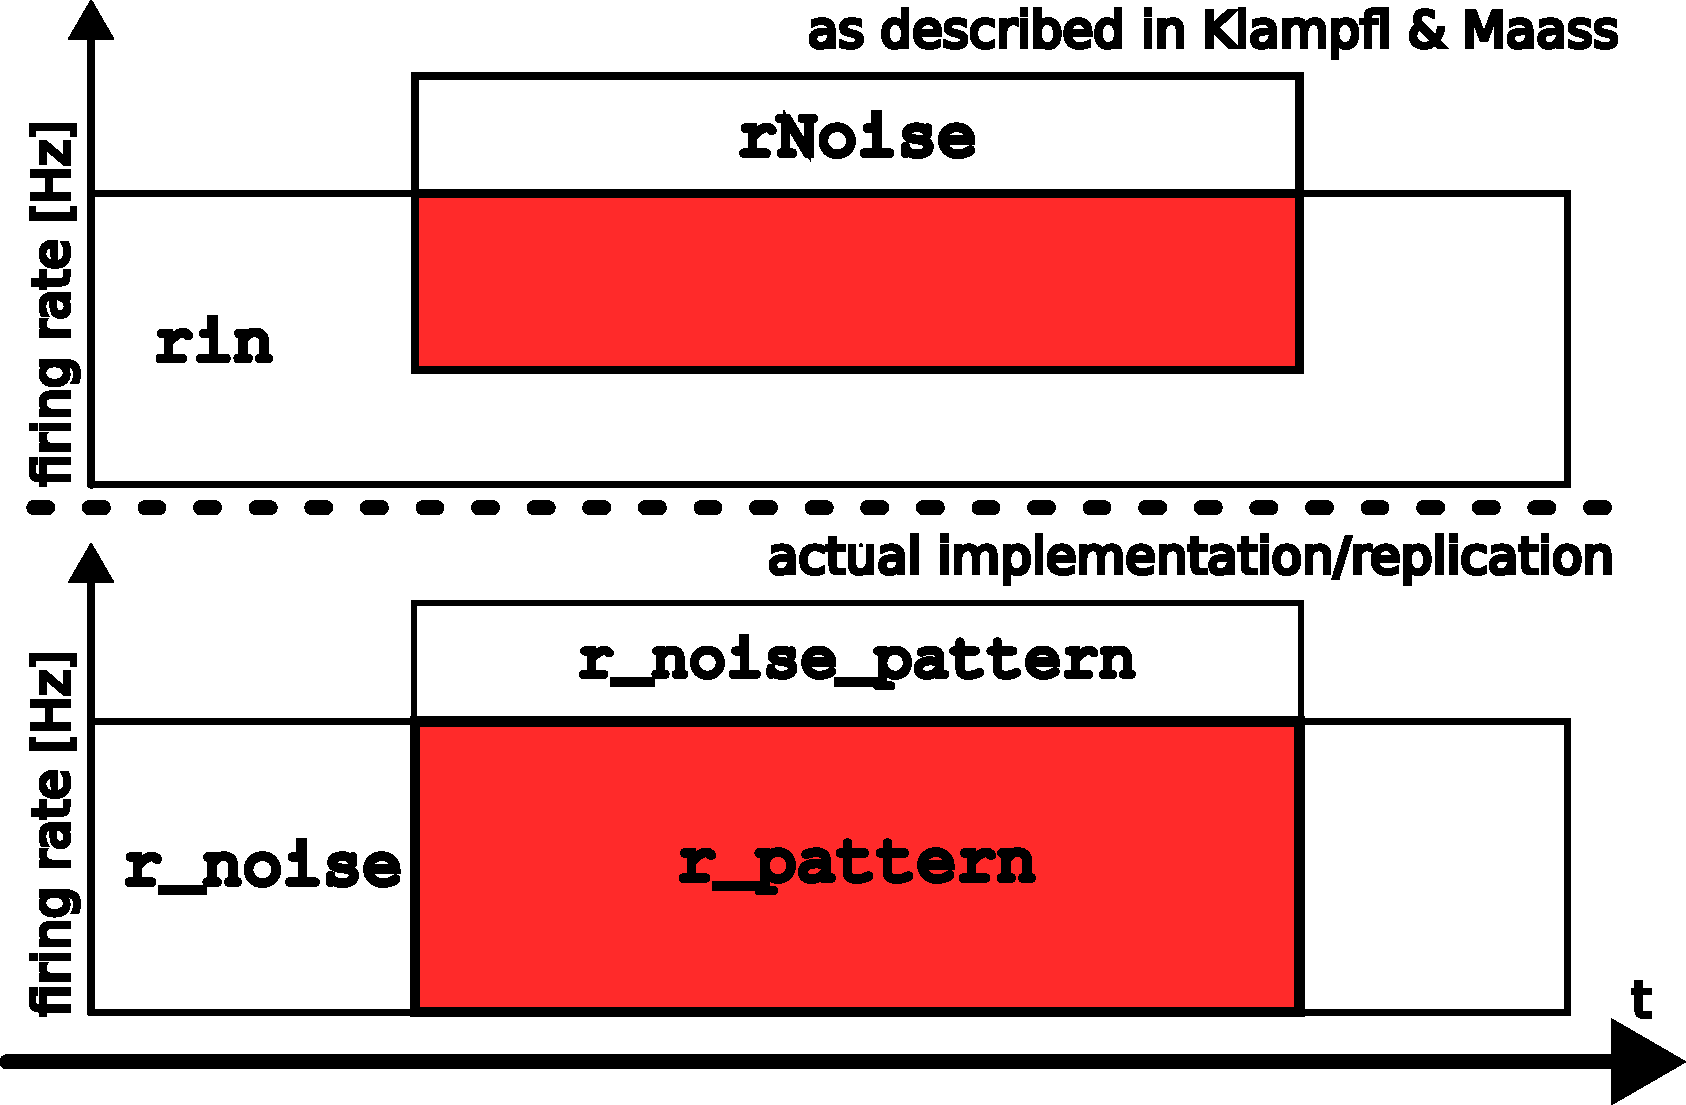
\includegraphics[width=0.9\columnwidth]{Figures/input_rates.pdf}
    \caption{Input rate comparison with pattern in red and noise in white}
    \label{fig:input_rates}
\end{figure}
\\
As mentioned earlier, different noise rates are needed for different time intervals. The reason for this is that unlike the distinction in "noise" and "pattern" phases might suggest, noise and pattern input are not mutually exclusive. In fact, pattern phases are usually superimposed with additional noise, requiring different noise rates during pattern presentation. There is however a difference between the reality of both the original and replicated implementation and the description from the paper as is illustrated in Figure \ref{fig:input_rates}. According to the description of Figure 4A in \parencite{klampfl_maass_2013}, a pattern of \SI{3}{\hertz} is embedded into an input spike train with constant rate \texttt{rin}=\SI{5}{\hertz} with additional \texttt{rNoise}=\SI{2}{\hertz} of noise laid over pattern presentations (Figure \ref{fig:input_rates} (top)). In the implementation of that same paper it was found however, that no embedding took place and the patterns had firing rate \SI{5}{\hertz}, just like \texttt{rin}.\\
The problem with the varying noise rates can be elegantly solved, since NEST provides a spike generator that offers a simple solution to this: the \textit{inhomogeneous\_poisson\_generator}. It generates Poisson noise of constant rate just like the regular \textit{poisson\_generator}, but in addition, allows for different noise rates at different intervals. This is used to specify two different noise rates: \texttt{r\_noise}, which is equivalent to \texttt{rin} during the noise phase, and \texttt{r\_noise\_pattern}, which is equivalent to the summed rate of \texttt{rNoise} and the noise remainder of \texttt{rin} during pattern presentation. This results in the same rate behavior and noise rate as in \parencite{klampfl_maass_2013}, while also taking advantage of NEST and simplifying the input generation.
\\ \ \\
With the groundwork of the \texttt{InputGenerator} described, the different possibilities for input generation and general procedure can be explained now with help from Figure \ref{fig:object_inputgenerator}. The general functioning of this is equivalent to the one described in Chapter \ref{sec:input_generation}. To tie in with the paragraph above, the different firing rates \texttt{r\_noise}, \texttt{r\_noise\_pattern}, \texttt{r\_input} can be freely set, as can be the number \texttt{n} of input channel assemblies from Figure \ref{fig:input_generator_structure}. It is however not required to play noise during simulation since it is determined by the value of \texttt{use\_noise}. To make the generator produce one or more input patterns or sequences of input patterns it has to be given the total number \texttt{n\_patterns} of different patterns it should create together with a duration for each of them in \texttt{t\_pattern}. These are created once by \texttt{create\_patterns()} and then stored for later use in \texttt{pattern\_list}.
The different sequences of patterns to present are contained \texttt{pattern\_sequences}, a list that specifies all possible compound sequences by the indices of patterns. A possible assignment for this could be [[0, 1], [2]], meaning that possible pattern combinations to present are pattern 0 directly followed by pattern 1 and pattern 2 alone. The order in which to present these sequences is determined by the sequence switching probability \texttt{p\_switch}, and \texttt{pattern\_mode}, which can be set to either of two modes \texttt{'random\_independent'} or \texttt{'random\_iterate'}. On \texttt{'random\_independent'} it selects the next sequence to present independently of previously played ones and on \texttt{'random\_iterate'} the next sequence from \texttt{pattern\_sequences} is presented with probability \texttt{p\_switch}, or the other way around, the current sequence is repeated with probability $1-$\texttt{p\_switch}.
\\ \ \\
The \texttt{InputGenerator} also stores information about the beginning of noise and pattern presentation phases that are used in the \texttt{Recorder} to order the spiking neuron output by mean activation time to make assemblies of neurons better recognizable. The data needed for this is stored in \texttt{phase\_times}, \texttt{pattern\_trace} and \texttt{next\_pattern\_length}.

\begin{figure}[htbp]
\centering
\begin{tikzpicture}
\begin{class}[text width=0.9\columnwidth]{InputGenerator}{0,0}
    \attribute{n: \textbf{int}}
    \attribute{target\_network: \textbf{NodeCollection}}
    \attribute{r\_noise: \textbf{int}}
    \attribute{r\_noise\_pattern: \textbf{int}}
    \attribute{r\_input: \textbf{int}}
    \attribute{n\_patterns: \textbf{int}}
    \attribute{pattern\_sequences: \textbf{list}}
    \attribute{pattern\_mode: \textbf{string}}
    \attribute{p\_switch: \textbf{float}}
    \attribute{t\_pattern: \textbf{list}}
    \attribute{t\_noise\_range: \textbf{list}}
    \attribute{pattern\_list: \textbf{list}}
    \attribute{spiketrain: \textbf{list}}
    \attribute{current\_pattern\_index: \textbf{list}}
    \attribute{spike\_generators: \textbf{NodeCollection}}
    \attribute{poisson\_generators: \textbf{NodeCollection}}
    \attribute{parrots: \textbf{NodeCollection}}
    \attribute{use\_noise: \textbf{bool}}
    \attribute{phase\_times: \textbf{list}}
    \attribute{pattern\_trace: \textbf{list}}
    \attribute{next\_pattern\_length: \textbf{list}}

    \operation{\_\_init\_\_(target\_network: \textbf{Network}, **kwargs) $\rightarrow$ \textbf{NoneType}}
    \operation{generate\_noise() $\rightarrow$ \textbf{NoneType}}
    \operation{create\_patterns() $\rightarrow$ \textbf{NoneType}}
    \operation{connect\_parrots() $\rightarrow$ \textbf{NoneType}}
    \operation{generate\_input(duration: \textbf{float}, t\_origin: \textbf{float}, force\_refresh\_patterns: \textbf{bool}) $\rightarrow$ \textbf{NoneType}}
    \operation{get\_next\_pattern\_id() $\rightarrow$ \textbf{int}}
    \operation{get\_patterns() $\rightarrow$ \textbf{list}}
    \operation{set\_patterns(patterns: \textbf{list}) $\rightarrow$ \textbf{NoneType}}
\end{class}
\end{tikzpicture}
\caption{\texttt{InputGenerator} Class Diagram} \label{fig:object_inputgenerator}
\end{figure}

%\begin{algorithm}
%	\caption{generate\_input(duration, t\_origin)} 
%	\begin{algorithmic}[1]
%	    \State t = 0
%	    \While{t < duration}
%	        \State t\_noise\_phase = random[t\_noise\_range]
%	        \For{ $i = 1,2,\dots, $n\_inputs}
%	            
%	        \EndFor
%	    \EndWhile
%	\end{algorithmic} 
%\end{algorithm}



\section{Recording and Measurement} \label{sec:recording}
\begin{figure}[htbp]
\centering
\begin{tikzpicture}
\begin{class}[text width=0.9\columnwidth]{Recorder}{0,0}
    \attribute{network: \textbf{Network}}
    \attribute{id\_list: \textbf{list}}
    \attribute{create\_plot: \textbf{bool}}
    \attribute{save\_figures: \textbf{bool}}
    \attribute{show\_figures: \textbf{bool}}
    \attribute{plot\_history: \textbf{bool}}
    \attribute{order\_neurons: \textbf{bool}}
    \attribute{dt\_rec : \textbf{int}}

    \operation{\_\_init\_\_(network: \textbf{Network}, id\_list: \textbf{list}, **kwargs)}
    \operation{set(**kwargs) $\rightarrow$ \textbf{NoneType}}
    \operation{run\_network() $\rightarrow$ \textbf{list}}
    \operation{record\_variables\_step() $\rightarrow$ \textbf{NoneType}}
    \operation{simulate(inpgen: \textbf{InputGenerator}, t: \textbf{int}, dt\_rec: \textbf{int}) $\rightarrow$ \textbf{NoneType}}
    \operation{get\_order(p: \textbf{list}, I: \textbf{list}, t: \textbf{list}, r\_fracs: \textbf{list}, tstart: \textbf{int}, nsteps: \textbf{int}) $\rightarrow$ \textbf{numpy.ndarray}}
\end{class}
\end{tikzpicture}
\caption{\texttt{Recorder} Class Diagram} \label{fig:object_recorder}
\end{figure}
The last object class on the Python level is the \texttt{Recorder}. While the other classes are mainly used for constructive work of the network, the \texttt{Recorder}s main function is to manage the simulation of that same network. For this it takes a \texttt{Network} object on construction with \texttt{\_\_init\_\_()}, along with an optional \texttt{id\_list} that contains the global IDs of the neurons from the \texttt{Network} that should be measured and plotted later as well as a set of self explanatory Boolean parameters (see Figure \ref{fig:object_recorder}) representing options for plotting outputs. Although these should be specified on initialization of a new \texttt{Recorder} object, all parameters can be changed later using the \texttt{set()} function. Since the \texttt{Recorder} handles simulation, the \texttt{run\_network()} function is its main function. It takes an \texttt{InputGenerator} (although this is optional) and simulates a network for a given period of time \texttt{t\_sim} with STDP/learning enabled or disabled, determined by the truth value of \texttt{train}. Because it is not always necessary or wanted to measure and plot the entire network, there are three different options besides recording the entire network:
\begin{enumerate}
    \item "Watch List": A list of neuron IDs \texttt{id\_list} to record from can be given to \texttt{run\_network()}. This is a good option for recording the same neurons over several network simulation sessions.
    \item "NodeCollection": A NodeCollection \texttt{node\_collection}, subset of the \texttt{Network} is specified and recorded.
    \item "Random $k$": $k$ neurons are randomly selected from the \texttt{Network} to record from. This is useful for creating a sample to record from in the very first simulation and then reusing the same sample in the "Watch List" mode.   
\end{enumerate} 
The general procedure of the \texttt{run\_network()} function starts by setting up recording devices, i.e. NEST \textit{multimeter} and \textit{spikerecorder} for the network and another separate \textit{spikerecorder} for the \texttt{InputGenerator}. The EPSPs and weights from the network are recorded by a separate \texttt{record\_variable\_step()} function by reading out network variables that were specifically made recordable to Python for this purpose in the C++ neuron model. Because reading out these variables does not work parallel to running the simulation, the simulation must be run in time steps of size \texttt{dt\_rec}. Setting this recording time window smaller will increase the resolution of the recording but comes with the trade-off of immensely deteriorated simulation efficiency and increased runtime.\\
After the setup of the recording devices, the actual simulation is run using the \texttt{simulate()} function that pre-generates the patterns of the \texttt{InputGenerator} for the duration of the simulation and then commands the NEST kernel to run the simulation for increments of \texttt{dt\_rec} and recording between increments until the NEST simulation has run for \texttt{t\_sim}. When the simulation and data collection are finished, the results are plotted. Optionally with neurons in the \textit{spikerecorder} readout ordered by their mean activation time during pattern presentation. This makes formed assemblies of neurons with related spiking behavior on input better visible.

\section{Neuron and Synapse Models} \label{sec:neuron_synapse_models}
As already mentioned in the Introduction, the models of the neuron and the synapse had to be implemented in C++ because NESTML did not provide the needed functionality. Before elaborating on the implementation, the concept of NEST synapse and neuron models needs to be explained. While in the original implementation all the neuron and synapse properties are handled in large arrays for the entirety of the network, in NEST each synapse and neuron is its own entity with a set of parameters. These entities are defined by models formulated in C++. Converting the original code into an object-oriented version proved to be very challenging and made it difficult to directly compare both implementations and detect errors. This will be covered in more detail in Chapter \ref{Chapter6}.

\subsection{Neurons} \label{ssec:neurons}
The custom neuron model follows a strict procedure to realize the same behavior as its non-object-oriented ancestor. The foundations of this procedure stem from NESTML \parencite{nestml_5_0_0}, although it was eventually abandoned as a modeling language. A neuron in NEST is generally updated on every simulation step, by the \texttt{update()} function, which first calls to \texttt{evolve\_epsps()} to update the current membrane potentials as described in Equations \ref{eqn:membrane_potential} and \ref{eqn:epsp}. Preceding that, input in the form of both \texttt{SpikeEvent}s and \texttt{InstantaneousRateConnectionEvent}s (described later) is managed by individual \texttt{handle()} functions. More precisely, on an incoming event of either kind, the properties of the spike are stored for later processing (e.g. by the \texttt{update()} function). 
\\ \ \\
%\subsubsection{Intermezzo: Operational Problems}
Implementing the membrane potential in NEST required a fair amount of creativity, given that Equation \ref{eqn:membrane_potential}, which defines it requires both the membrane potentials from all other neurons in the same WTA (although NEST neuron models have no concept of such things as WTAs) and the weights from all incoming synapses, which is not conventionally available from the postsynaptic neuron since it is a property of the synapse. These two problems made it entirely impossible to implement the model in NESTML, making the implementation even more complex and time-consuming, since the model now had to be manually written in C++ without the help of a modeling language, which was not intended when planning this thesis.\\
As already alluded to before, the problem of communicating the membrane potential (needed for calculating the summed firing rate of the WTA), was solved by introducing a new connection type already existing in NEST called \texttt{rate\_connection\_instantaneous}. Because it was originally designed for connecting rate model neurons it had to be modified to send and receive membrane potentials instead of firing rates. These connections are created \textit{all-to-all} (excluding self loops) between the neurons in the same WTA by the \texttt{form\_WTA} function on the Python level.\\
The second problem about the synapse weights was solved by creating a new internal vector \texttt{localWeights\_Wk} that was initialized with length $1000$ and filled with $0$ on construction. Setting the length fixed to $1000$ is not a perfect solution because this also means that for now, each neuron can only have as much as $1000$ presynaptic neurons and if it has less there may be a considerable overhead slowing down the simulation and wasting space. This can likely be fixed by using vectors of dynamic sizes and initializing them on network creation before the simulation starts. But since this was not a priority and did not cause problems for now, this remains to be implemented at a later point in time.
\\ \ \\
Following the calculation of membrane potential, \texttt{evolve\_epsps()} also updates the decay-time EPSP and rise-time EPSP from Equation \ref{eqn:epsp} using the update rule found in the original code (Equation \ref{eqn:epsp_update}). After the current membrane has been determined this way, the firing rate is set as defined in Equation \ref{eqn:firing_rate_paper}, with two additions. The first is that the term to calculate a neuron's fraction of firing rate in the WTA
\begin{equation*}
    \texttt{rate\_fraction}_k(t)=\frac{\exp(u_k(t))}{\sum_{j=1}^K\exp(u_j(t))}
\end{equation*}
is stored in a variable for use in the ordering function to later sort the neurons by mean activation time for better identifiability of output assemblies. The second is that the firing rate of the neuron is set to $0$ if the above rate fraction is larger than $1$. This should be impossible, but it has been found that due to an issue with the value initialization in NEST this can occur and tamper with the correct results. Setting the rate to $0$ temporarily is not technically conform with the precise model definition, but this sacrifice is justified considering it replaces a more destructive inconsistency and could not be found to alter the simulation results in any meaningful way in comparison with the original as will be shown in Chapter \ref{Chapter5}.\\
To make the neuron fire with the calculated firing rate a firing probability
\begin{equation*}
    p_{spike}(\texttt{rate})=\texttt{resolution}\cdot \frac{\texttt{rate}}{1000}
\end{equation*}
is calculated from it and with that same probability, a spike is then scheduled to be emitted in the next simulation step by \texttt{set\_spiketime}. The \texttt{resolution} here refers to the simulation time step size (set to \SI{1}{\milli\second}). Additionally, the weights are also updated by the STDP rule (Equation \ref{eqn:stdp_real}, including variance tracking from Equations \ref{eqn:variance_tracking}, \ref{eqn:variance_tracking_2}) when a spike is emitted, since STDP weight update should only occur on a firing postsynaptic neuron (the weight update is turned off when learning is disabled though, e.g. during testing of a trained network). The reason the STDP weight update is performed in the neuron rather than the synapse is related to the previously described problem of calculating the membrane potential. Because the weights updated by STDP are needed for this equation and it uses the \texttt{localWeights\_Wk} instead of the synapse weights, the STDP has to use them as well.\\
In the end of the \texttt{update()} procedure, the outgoing membrane potential communication is handled by sending an \texttt{InstantaneousRateConnectionEvent} (which is transmitted over the \texttt{rate\_connection\_instantaneous} connection) with the current membrane potential of the neuron.

\subsection{Synapses} \label{ssec:synapses}
Since most aspects of the complete model, including a lot of the synapse logic, are already implemented in the NEST neuron model, the functionality covered by the synapse is decidedly smaller. An individual synapse in NEST is also accessed less frequently than a neuron because while the neuron gets updated every simulation step, the synapse is only updated on activity, i.e. when the presynaptic neuron fires. The only key characteristic from the original model it implements is the STP, which is calculated as defined by Equation \ref{eqn:stp}. 

% recordables
% V_, S_, P_
% parameters are set once and not changed during simulation or ever

\section{Summary of Complications} \label{sec:summary_complications_implementation}
Similar to Section \ref{sec:summary_complications_original}, this section briefly summarizes critical problems with NEST that hindered the construction of the replication.
\begin{itemize}
    \item communication of voltages within definable NodeCollections (for\linebreak WTAs) is not supported by NEST. This required handcrafting a new connection type and embedding it into the neuron and synapse model (see Section \ref{ssec:neurons}).
    \item fetching the identity of the presynaptic neuron on spike arrival at the postsynaptic neuron is not natively supported by NEST
    \item managing synaptic weights from their postsynaptic neuron as required for the implementation of the model is also not natively supported by NEST
\end{itemize}


% Chapter Template

\chapter{Results \& Comparison} % Main chapter title

\label{Chapter5} % Change X to a consecutive number; for referencing this chapter elsewhere, use \ref{ChapterX}


To verify the correctness of the new implementation, it will be compared to the original implementation from \parencite{klampfl_maass_2013}, starting with toy models to prove equal behavior on the smallest possible level and proper functioning of individual properties like plasticity and lateral inhibition (Section \ref{sec:toy_models}). After that, the tested network's size will be increased until the parameters of the full-scale model described in Figure 4 of \parencite{klampfl_maass_2013} are reached (Section \ref{sec:full_scale}).

\section{Toy Models} \label{sec:toy_models}
%\begin{table}[]
%\begin{tabular}{|l|lllllll|}
%\hline
%Test & Grid size   & $K$ & lateral inhibition & STDP & STP & Rate & Input rate \\
%\hline
%1A   & $1\times 2$ & 1   & Off                & On   & Off & 50   & 60         \\
%1B   & $1\times 2$ & 1   & Off                & On   & Off & 100  & 2          \\
%2    & $1\times 2$ & 2   & On                 & On   & Off & 50   & 20         \\
%3    & $1\times 2$ & 2   & On                 & On   & On  & 50   & 20         \\  
%\hline
%\end{tabular}
%\end{table}
%%%%%%%%%%%%%%%%%%%%%%%%%%%%%%%%%%%%%%%%%%%%%%%%%%%%%%%%%%%%%%%%%%%%%%%%%%%%%%%%%%%%%%%
\subsection{Baseline Test} \label{ssec:baseline_test}
\begin{figure}[htbp]
    \centering
    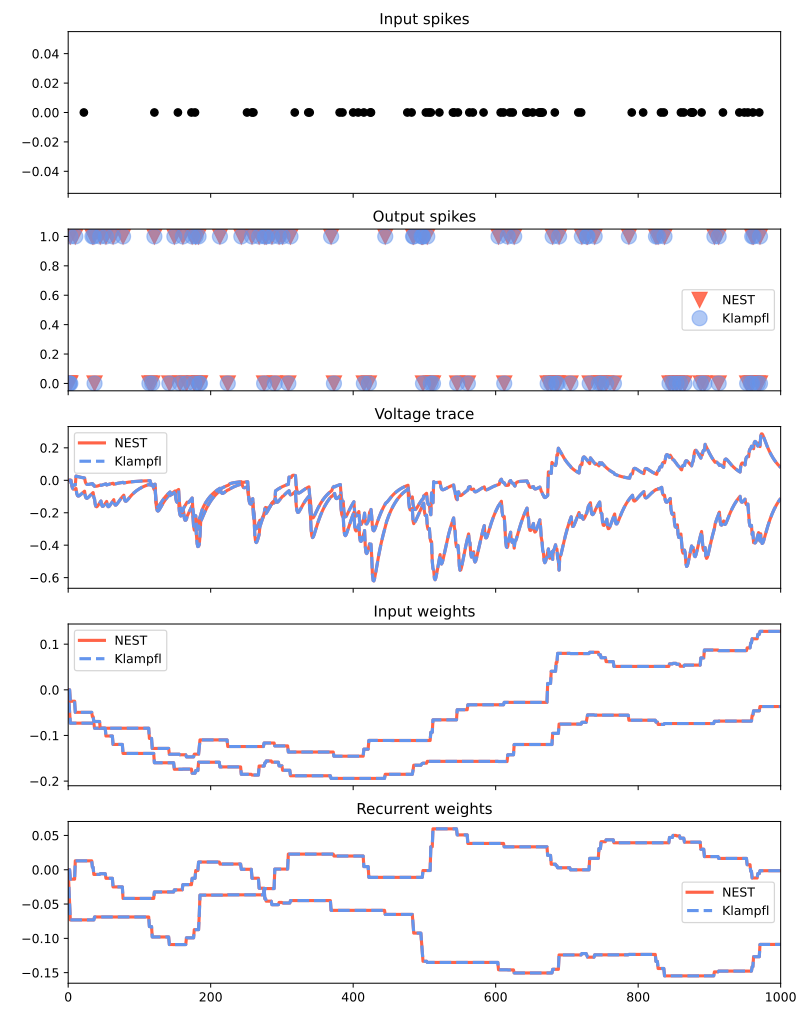
\includegraphics[width=\columnwidth]{Figures/joint_tm_2wta1.png}
    \caption{Toy Model: Test of $1\times 2$ WTA grid with $k=1$ and one input channel for \SI{1}{\second}. Input and output spikes are fixed at \SI{60}{\hertz} and \SI{50}{\hertz}. STP is disabled.}
    \label{fig:joint_tm_2wta1_A}
\end{figure}
\begin{figure}[htbp]
    \centering
    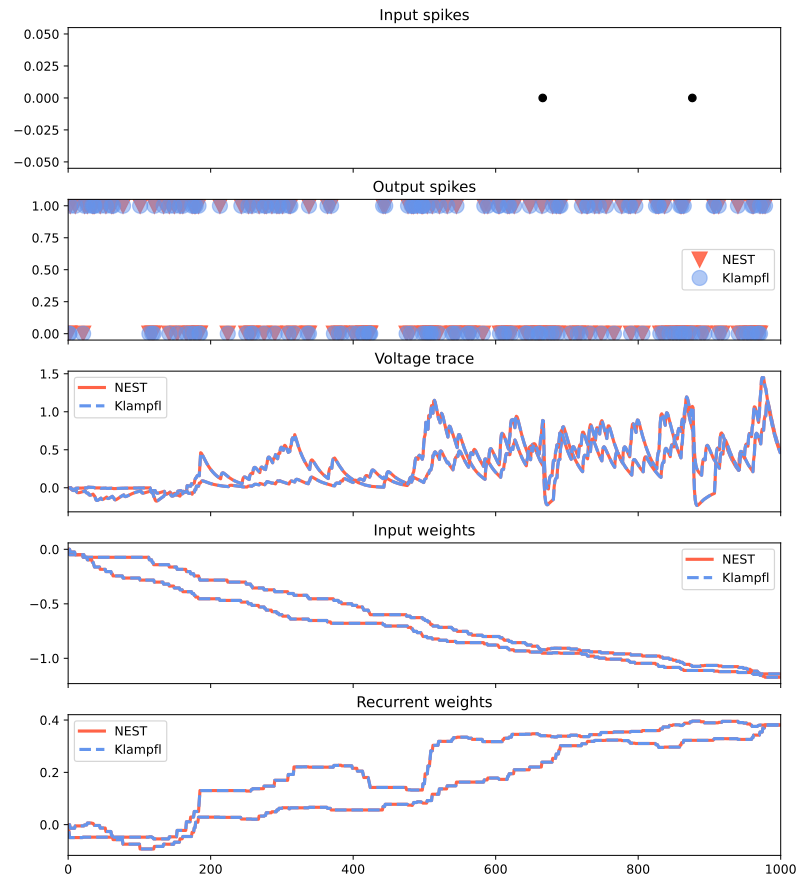
\includegraphics[width=\columnwidth]{Figures/joint_tm_2wta1_B.png}
    \caption{Toy Model: Test of $1\times 2$ WTA grid with $k=1$ and one input channel for \SI{1}{\second}. Input and output spikes are fixed at \SI{2}{\hertz} and \SI{100}{\hertz}. STP is disabled.}
    \label{fig:joint_tm_2wta1_B}
\end{figure}
To start off, a minimal network of grid size $1\times2$, in which each WTA contains just one neuron will be tested for a singular input source over \SI{1000}{\milli\second}. The WTA size is set to $1$ to bypass the effect of lateral inhibition. STP is also disabled, leaving only STDP as a dynamic network property to test. The purpose of this test is to prove the equal behavior of both implementations, which is why the embedded stochastic firing behavior of both implementations is turned off and replaced with predefined spike times, both for neuron in- and output, which were generated randomly and set to be identical for both programs externally. For the input firing rate and neuron firing rate \SI{50}{\hertz} and \SI{60}{\hertz} were chosen respectively.\\
The results of this test can be seen in Figure \ref{fig:joint_tm_2wta1_A}, where the pre-generated in- and output spikes are visualized along with the weights of the incoming and recurrent synaptic connections within the network and the resulting membrane potential ("Voltage trace").\\
From these results, we can conclude that since the plotted traces for both programs do not deviate from one another, the behavior of STDP and membrane potential in this context without lateral inhibition and STP is identical for original and replication. And since the membrane potential is computed as the sum of the EPSP scaled by the respective synaptic weights, this implies also that the EPSPs are identical. But more can be deduced from the same test setup by changing the firing rates to \SI{2}{\hertz} for input and \SI{100}{\hertz} for recurrent output spiking (Figure \ref{fig:joint_tm_2wta1_B}). With neither STP nor lateral inhibition at work, weights can switch signs depending on the rate of the external input and output firing rates of the neurons. This also shows that Dale's principle (described in Chapter \ref{Chapter2}) 
is not preserved when using STDP and STP disabled, since both inhibition and excitation of neurons by the same entities are possible, which is proven by the voltage traces of Figure \ref{fig:joint_tm_2wta1_A} and \ref{fig:joint_tm_2wta1_B} developing toward both positive and negative values. That being said, Dale's principle is not enforced in this model in any way, i.e. the weights are not bound to a specific interval during learning.

%%%%%%%%%%%%%%%%%%%%%%%%%%%%%%%%%%%%%%%%%%%%%%%%%%%%%%%%%%%%%%%%%%%%%%%%%%%%%%%%%%%%%%%
\subsection{Scaled WTA Test}
\label{ssec:lateral_inhibition_test}
\begin{figure}[htbp]
    \centering
    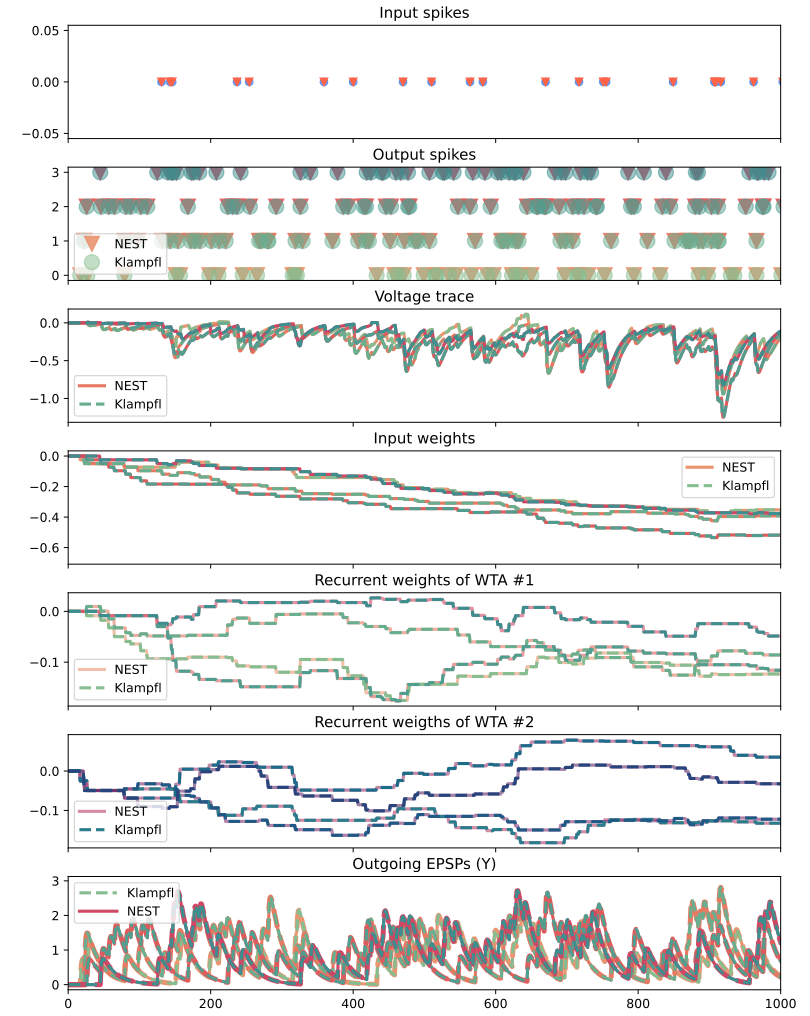
\includegraphics[width=\columnwidth]{Figures/joint_tm_2wta2.png}
    \caption{Toy Model: Test of $1\times 2$ WTA grid with $k=2$ and one input channel for \SI{1}{\second}. Input and output spikes are fixed at \SI{20}{\hertz} and \SI{50}{\hertz}. STP is disabled.}
    \label{fig:joint_tm_2wta2}
\end{figure}
The second test (Figure \ref{fig:joint_tm_2wta2}) serves as an intermediate test for later comparison. It increases the WTA size from $1$ in the last test to $2$ and also adds a plot for EPSPs.
This setup allowed testing the \texttt{rate\_connection\_instantaneous} along with the rate normalization in general, more specifically if the values of the \texttt{rate\_fraction}s were computed correctly. Most parameters are taken from \ref{ssec:baseline_test}, except for the fixed firing rates, which were set to \SI{50}{\hertz} and \SI{20}{\hertz} for recurrent and input firing rate respectively. Original and replication still produce identical results. 

%%%%%%%%%%%%%%%%%%%%%%%%%%%%%%%%%%%%%%%%%%%%%%%%%%%%%%%%%%%%%%%%%%%%%%%%%%%%%%%%%%%%%%%
\subsection{STP Test} \label{ssec:stp_test}
\begin{figure}[htbp]
    \centering
    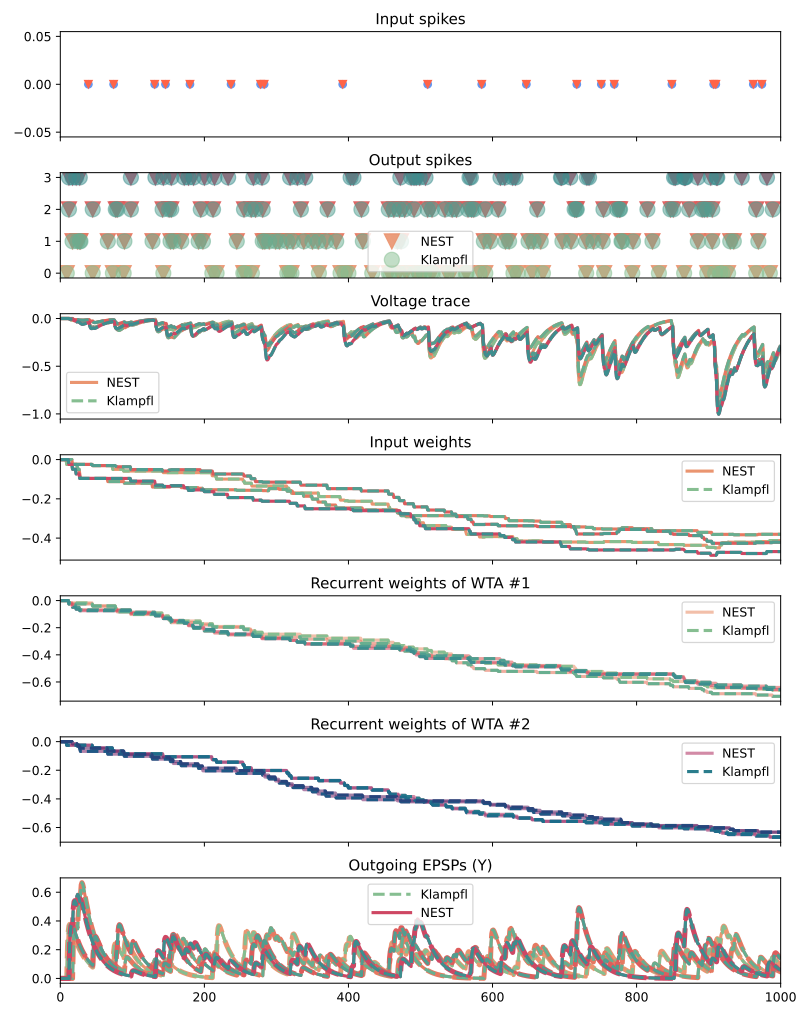
\includegraphics[width=\columnwidth]{Figures/joint_tm_2wta2_stp.png}
    \caption{Toy Model: Test of $1\times 2$ WTA grid with $k=2$ and one input channel for \SI{1}{\second}. Input and output spikes are fixed at \SI{20}{\hertz} and \SI{50}{\hertz}. STP is enabled.}
    \label{fig:joint_tm_2wta2_stp}
\end{figure}
For the next test, all parameters stay the same as in \ref{ssec:lateral_inhibition_test}, except for STP which is now enabled, producing the plot in Figure \ref{fig:joint_tm_2wta2_stp} and allowing a comparison of network behavior with and without STP in combination with Figure \ref{fig:joint_tm_2wta2}. Notice that the addition of STP makes the recurrent weights diverge to the negative range and stabilizes the membrane potential to the negative range, whereas the voltage trace without STP contained positive valued outliers. However, weight and voltage adjustments are just the secondary effects of the EPSP being directly affected by STP, vastly reducing its maximum excitability.


%%%%%%%%%%%%%%%%%%%%%%%%%%%%%%%%%%%%%%%%%%%%%%%%%%%%%%%%%%%%%%%%%%%%%%%%%%%%%%%%%%%%%%%%%%
%%%%%%%%%%%%%%%%%%%%%%%%%%%%%%%%%%%%%%%%%%%%%%%%%%%%%%%%%%%%%%%%%%%%%%%%%%%%%%%%%%%%%%%%%%
%%%%%%%%%%%%%%%%%%%%%%%%%%%%%%%%%%%%%%%%%%%%%%%%%%%%%%%%%%%%%%%%%%%%%%%%%%%%%%%%%%%%%%%%%%
\section{Full Scale Network} \label{sec:full_scale}
\subsection{Formation of Assemblies}
With the accuracy of the implementation proven for all major components of the model, it can now be compared if the full-scale models still produce the same results. For testing larger models, fixing random numbers between implementations becomes prohibitive, meaning that these tests' results are not expected to be identical and should rather show the same qualitative behavior. For the following tests, networks with the following properties will be compared in Figure \ref{fig:nest_full_scale} and \ref{fig:legacy_full_scale}:\\
\begin{table}[h!]
\begin{tabular}{|ll}
Grid size            & $10\times 5$                                       \\
WTA size range       & [2; 10]                                            \\
\#Input channels     & 100                                                \\
Training time        & \SI{100}{\second}                                  \\
Testing time         & \SI{3}{\second}                                    \\
\#Patterns           & 1                                                  \\
Noise duration range & [\SI{300}{\milli\second}; \SI{500}{\milli\second}] \\
Pattern duration     & \SI{300}{\milli\second}                       
\end{tabular}
\end{table}

\begin{figure}[htbp]
    \centering
    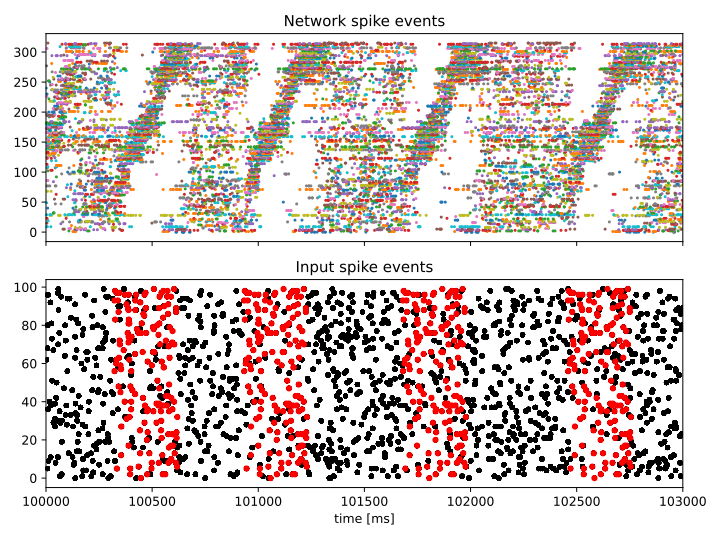
\includegraphics[width=\columnwidth]{Figures/nest_full_scale.png}
    \caption{Full-scale Network: NEST \SI{3}{\second} test after \SI{100}{\second} training}
    \label{fig:nest_full_scale}
\end{figure}
\begin{figure}
    \centering
    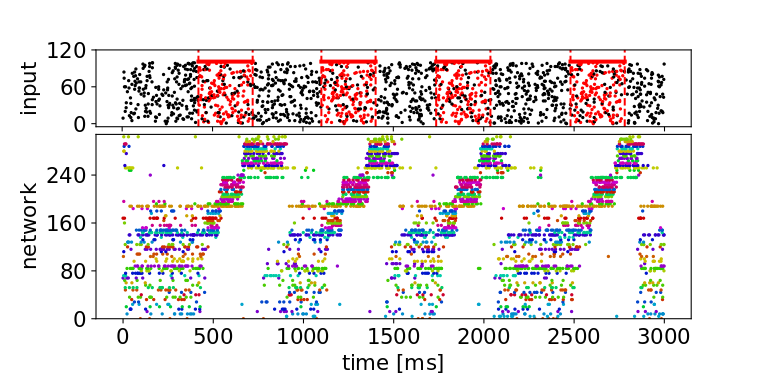
\includegraphics[width=\columnwidth]{Figures/legacy_full_scale.png}
    \caption{Full-scale Network: Legacy \SI{3}{\second} test after \SI{100}{\second} training. Only 100 neurons plotted to reduce clutter in network spikes plot.}
    \label{fig:legacy_full_scale}
\end{figure}

\subsection{Necessity of Variance Tracking}
During testing of the original implementation, it was also found that variance tracking was in fact crucial to the learning capabilities of the model as can be seen in Figure \ref{fig:variance_tracking_comparison}. This figure shows the results of two \SI{3}{\second} testing runs of the network each following a \SI{100}{\second} training phase. During the training phase a network of grid size $10\times 5$ and $k\in[2; 10]$ with $100$ input channels was fed with a \SI{5}{\hertz} of either pattern input (shown in red) or noise input (black), with \SI{2}{\hertz} of noise additionally laid over each pattern phase. As can clearly be seen, if variance tracking is enabled, assemblies of neurons with similar spike characteristics emerge as a consequence of pattern input, while disabling variance tracking prevents the formation of such assemblies. From this follows that variance tracking as described in \parencite{nessler_et_al_2013} is a requirement for learning in \parencite{klampfl_maass_2013}, while the STDP rule from Equation \ref{eqn:stdp_real} alone does not appear to be able to make such learning possible.\\
This phenomenon can also be replicated in the NEST implementation as demonstrated in Figure \ref{fig:nest_full_scale_no_variance_tracking}.
\begin{figure}[htbp]
    \centering
    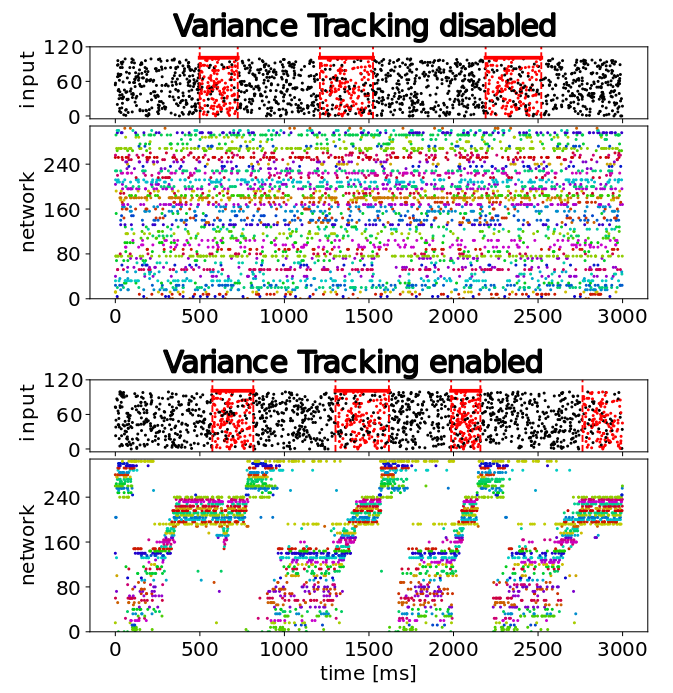
\includegraphics[width=0.8\columnwidth]{Figures/variance_tracking_comparison.png}
    \caption{Full-scale Network: Legacy \SI{3}{\second} test after \SI{100}{\second} simulation with and without variance tracking}
    \label{fig:variance_tracking_comparison}
\end{figure}
\begin{figure}[htbp]
    \centering
    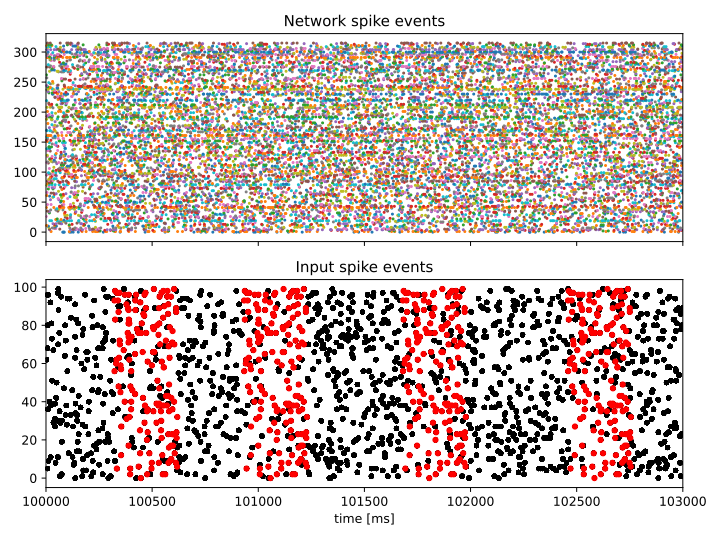
\includegraphics[width=0.85\columnwidth]{Figures/nest_full_scale_no_variance_tracking.png}
    \caption{Full-scale Network: NEST \SI{3}{\second} test after \SI{100}{\second} training without variance tracking}
    \label{fig:nest_full_scale_no_variance_tracking}
\end{figure}

\subsection{Necessity of STP}
For the following test, STP will be turned off for testing its effect on long-term network spike behavior. In \parencite{klampfl_maass_2013} Figure 6A a similar test is conducted with a slightly different testing setup in the "without depressing synapses" panel, which means nothing else than "without STP". As can be seen when comparing Figure \ref{fig:nest_full_scale_no_stp} to the Figure in \parencite{klampfl_maass_2013}, the behavior without STP is comparable in both cases.
\begin{figure}[htbp]
    \centering
    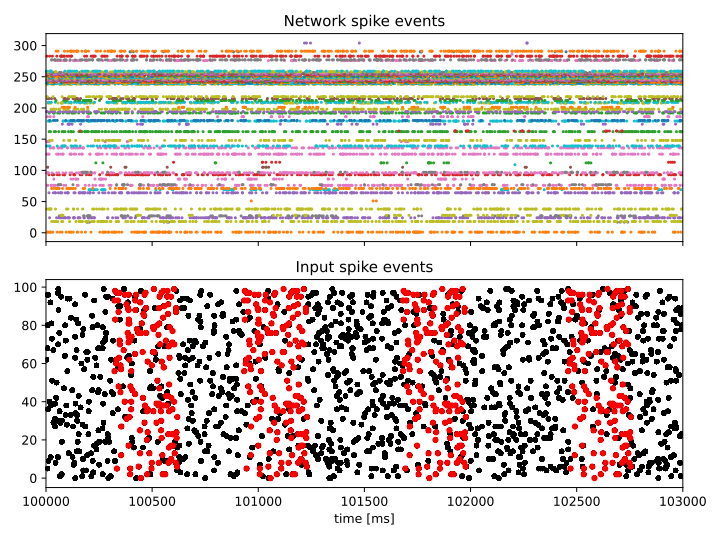
\includegraphics[width=\columnwidth]{Figures/nest_full_scale_no_stp.png}
    \caption{Full-scale Network: NEST \SI{3}{\second} test after \SI{100}{\second} training without STP}
    \label{fig:nest_full_scale_no_stp}
\end{figure}

\subsection{Performance Benchmarking}
An important asset of the NEST implementation that has not yet been mentioned is its vastly superior performance. This is an effect of the more efficient simulation kernel of NEST, whereas the version of Klampfl and Maass simulates stepwise and uses matrix multiplication for calculation. In the table below the real-time factors of simulations for both implementations are benchmarked for the full-scale model task from Section \ref{sec:full_scale}. The hardware used for benchmarking is a Lenovo YOGA 730-15IWL Notebook with 16GB of memory, an Intel Core i7-8565U CPU with 8 cores, and running Ubuntu 22.04 LTS. The original implementation will use all cores while the NEST implementation here only uses 6 cores.
\begin{table}[htbp]
\centering
\begin{tabular}{|l|l|l|}
\hline
       & Real-time factor & Simulation Time                                     \\ \hline
NEST   & 0.7362           & \SI{73.63}{\second}                                 \\
Legacy & 41.83            & \SI{69}{\minute} \SI{43}{\second} = \SI{4183}{\second} \\ \hline
\end{tabular}
\end{table}

\section{Further Experiments}
\begin{figure}[htbp]
    \centering
    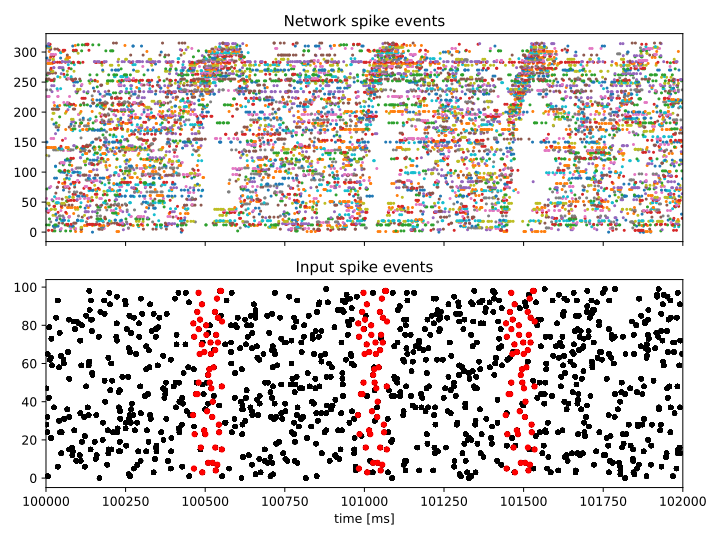
\includegraphics[width=\columnwidth]{Figures/nest_experiment_100ms.png}
    \caption{Pattern duration set to \SI{100}{\milli\second}. Grid size $10\times 5$ with $k\in[2;10]$ and 100 input channels. Input rate of \SI{5}{\hertz} with additional \SI{2}{\hertz} during pattern presentation. \SI{2}{\second} test after \SI{100}{\second} training.}
    \label{fig:nest_experiment_100ms}
\end{figure}
To test a few of the boundaries of the replicated model, the pattern duration was varied to examine the assembly formation under these conditions. Figure \ref{fig:nest_experiment_100ms} shows the results of a pattern duration of \SI{100}{\milli\second} and Figure \ref{fig:nest_experiment_900ms} shows the result of a pattern duration of \SI{900}{\milli\second}. The first visible difference between short and long duration is the size of the formed assembly. Where the long pattern activates almost the entire network over time, the shorter pattern activates a much smaller assembly. This also comes with different levels of assembly distinction. The short pattern causes a clear phase of inactivity for a part of the network, while the longer pattern already activates the whole network, preventing parts of it to become inactive and therefore impeding learning.
\\ \ \\
In both cases conclusions are deducible: Too long patterns cannot be learned by the network because they overstimulate it, preventing assemblies of reduced activity during pattern presentation to form. Too short patterns on the other hand can only excite small assemblies, to the point where they will not have a noticeable effect at all.
\begin{figure}[htbp]
    \centering
    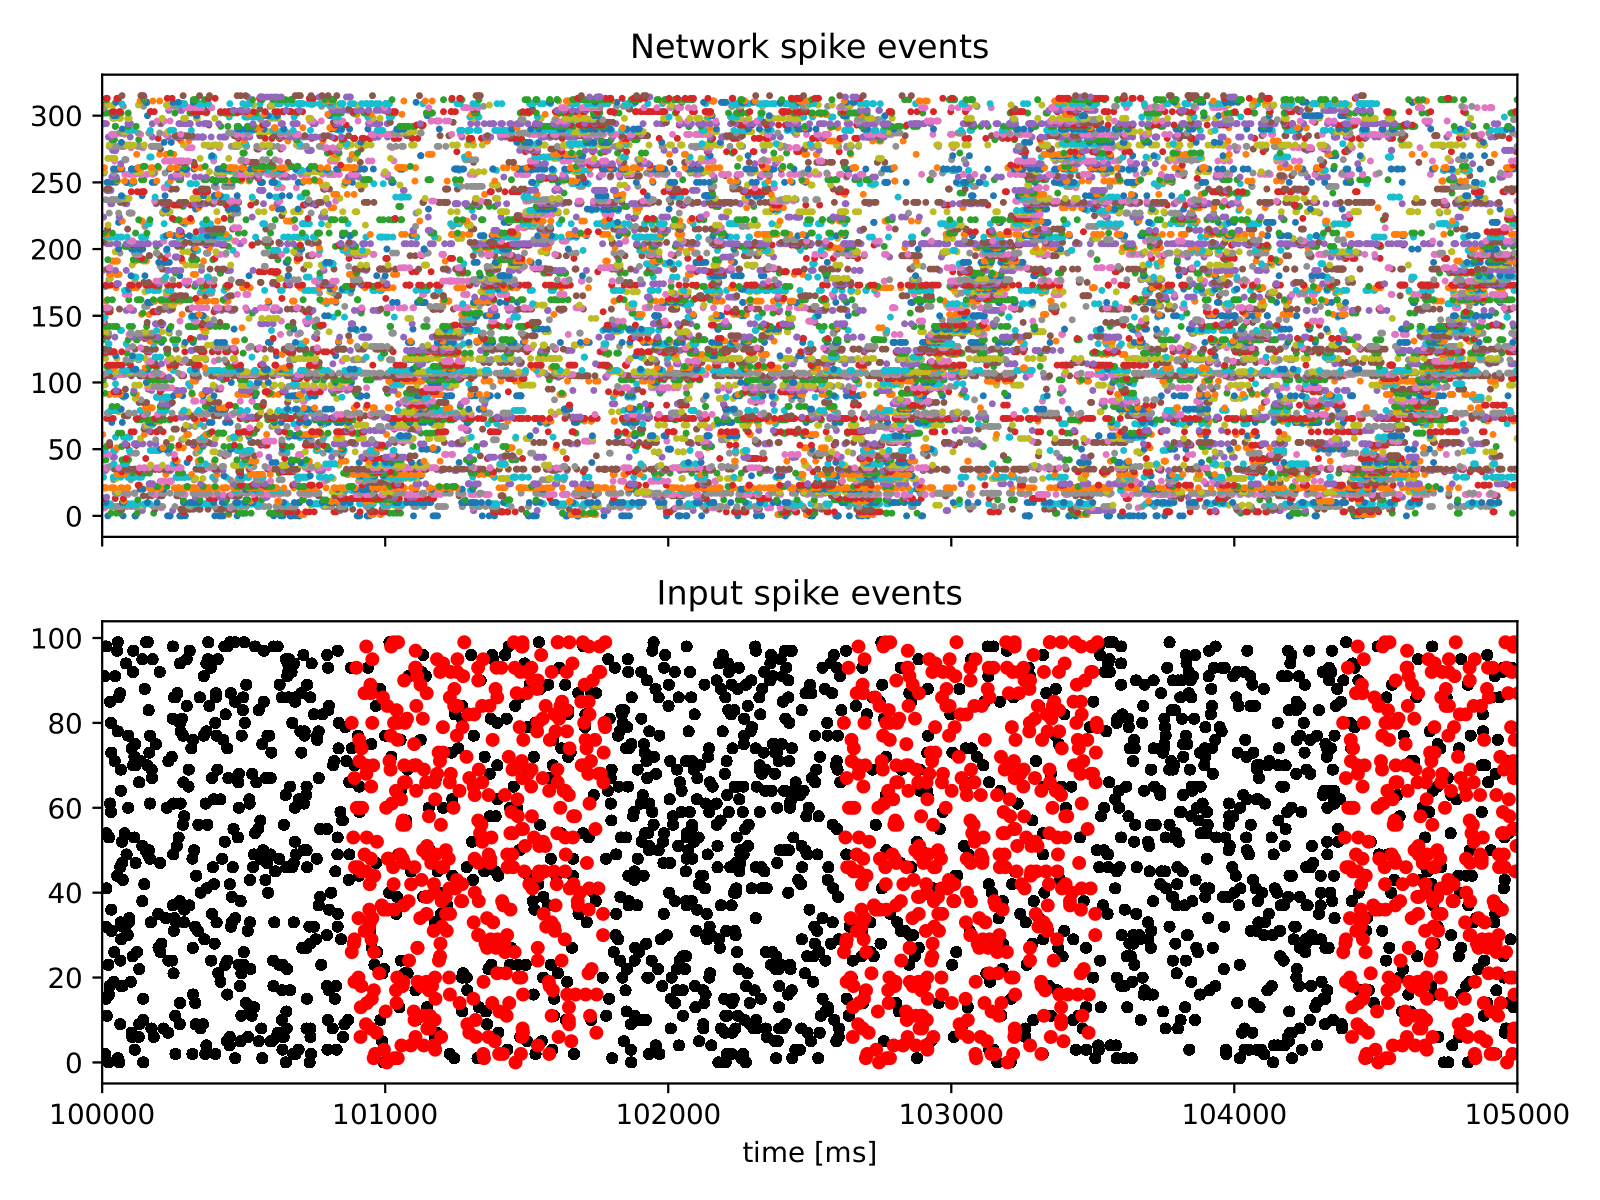
\includegraphics[width=\columnwidth]{Figures/nest_experiment_900ms.png}
    \caption{Pattern duration set to \SI{900}{\milli\second}. Grid size $10\times 5$ with $k\in[2;10]$ and 100 input channels. Input rate of \SI{5}{\hertz} with additional \SI{2}{\hertz} during pattern presentation. \SI{5}{\second} test after \SI{100}{\second} training.}
    \label{fig:nest_experiment_900ms}
\end{figure}






% describe edge case behavior and capabilities of NEST implementation. e.g.:
% prolongated pattern duration (>600ms) to test how much the model can learn
% different patterns



% referring back to the postulated constraint 2. from the Introduction (Chapter \ref{Chapter1}) it is tested if STDP between PCs is needed for required for the formation of spiking assemblies in both the klampfl-maass implementation and the new one


% Chapter Template

\chapter{Conclusion} % Main chapter title

\label{Chapter6} % Change X to a consecutive number; for referencing this chapter elsewhere, use \ref{ChapterX}

%----------------------------------------------------------------------------------------
%	SECTION 1
%----------------------------------------------------------------------------------------

\section{Conclusion}
While this thesis ran into many unforeseeable obstacles, most of the goals set for it were eventually achieved. This allows to draw several conclusions:
\\ \ \\
The original model has limited implementability when using an object-oriented approach and dedicated neural simulator such as NEST because many equations describing the model behavior require information to be globally available that is not usually disclosed to all entities described by the model. The most prominent example of this being the availability of synaptic weights at the postsynaptic neuron, as described in \ref{ssec:neurons}. When using NEST, it would be more favorable to select a different model for replication that can be integrated better, especially concerning the calculation of membrane potential. Also, it became clear that writing more complicated NEST neuron and synapse models by hand is very prone to bugs and errors because the code gets cluttered very fast and may provoke rare and hard-to-find bugs in NEST because NEST can not possibly provide universal support for every implementation approach chosen by developers.
\\ \ \\
Despite the difficulty replicating the model in NEST, the process eventually was successful and rewarding. Most remarkable perhaps is the superiority in simulation speed, benchmarked at over a 55-fold speedup compared to the original, making it faster than real-time for many tests. This speedup allows a more flexible use of the model for testing. Also, the replication successfully uncovered many details and hidden assumptions about \parencite{klampfl_maass_2013} that can now be considered for future work with related models to avoid similar problems.

\section{Future Work}
As the complexity of this work and its implementation increased continuously throughout its processing, there are several possible directions for future work based on this work. 
For one, there were a few smaller details about the original paper pointed out, like the incorrect adoption of the STP equation from \parencite{markram_wang_tsodyks_1998}. It should be ensured that the change introduced by \parencite{klampfl_maass_2013} does not affect the correctness or characteristics of the STP.\\
Another point of interest would be the abstract implementation of lateral inhibition. It is clear that the normalization of the firing rate in each WTA is not biologically plausible behavior, although \parencite{klampfl_maass_2013} pointed out that it did not affect their results in a meaningful way. Nevertheless, if this model should be used for further research and especially for tests that Klampfl and Maass did not design this model for, a more biologically accurate implementation of lateral inhibition should be deployed. A suitable approach for this could be created using the model from \parencite{häusler_maass_2017}, where lateral inhibition is described in a more detailed way and using two different types of inhibition, implemented by two different populations of inhibitory neurons, one for rate normalization and the other for blocking STDP.\\
Due to the limited time of the thesis, there also remain more tests from \parencite{klampfl_maass_2013} itself, where more advanced input is presented to the network and even nonlinear computing tasks like XOR are solved.

% Test setup, Analysis, 



%----------------------------------------------------------------------------------------
%	THESIS CONTENT - APPENDICES
%----------------------------------------------------------------------------------------

\appendix % Cue to tell LaTeX that the following "chapters" are Appendices

% Include the appendices of the thesis as separate files from the Appendices folder
% Uncomment the lines as you write the Appendices

% Appendix Template

\chapter{Glossary of Notations} % Main appendix title

\label{AppendixX} % Change X to a consecutive letter; for referencing this appendix elsewhere, use \ref{AppendixX}
\begin{table}[htbp]
\begin{tabular}{|l|l|}
\hline
Mathematical   & Meaning                                                 \\
\hline
$w_{ki}$       & Weight of synaptic connection from neuron $z_i\rightarrow z_k$     \\
$u_k$          & dynamic facilitation variable of neuron $k$             \\
$R_k$          & dynamic depression variable of neuron $k$               \\
$U$            & STP parameter                                           \\
$D$            & Depression time constant                                \\
$F$            & Facilitation time constant                              \\
$\tau_{rise}$  & Rise time constant of EPSP                              \\
$\tau_{decay}$ & Decay time constant of EPSP                             \\
$r_k(t)$       & Firing rate of neuron $k$ at time $t$                   \\
$u_k(t)$       & Membrane potential of neuron $k$ at time $t$            \\
$y_i(t)$       & EPSP of neuron $i$ at time $t$                          \\
$R_{\max}$     & Maximum firing rate of a WTA circuit                    \\
$\Delta_{k-1}$ & Interspike interval between spikes $k$ and $k-1$        \\
$\eta_{ki}$    & Adaptive learning rate of synapse from neuron $z_i\rightarrow z_k$ \\
$A_{k}$        & Amplitude of the $k$-th input spike                     \\
$c$            & Scaling constant for controlling the strength of STDP   \\
$w_{k0}$       & Bias/excitability parameter of neuron $k$               \\
$K$            & Number of neurons in a WTA circuit                      \\ 
$z_k$          & $k$-th neuron in a WTA circuit                          \\
$\lambda$      & Parameter of exponential distance distribution          \\
\hline
\end{tabular}
\caption{Glossary of mathematical notations}
\label{tab:mathematical_notations}
\end{table}

\begin{table}[htbp]
\begin{tabular}{|l|l|l|l|}
\hline
Mathematical   & Original & Replication          & Value                                                                \\
\hline
$r_k(t)$       & -        & r                    & Equation \ref{eqn:firing_rate_paper}                                 \\
$R_{\max}$     & rmax     & R\_max               & \SI{100}{\hertz}                                                     \\
$u_k(t)$       & u        & V\_m                 & Equation \ref{eqn:membrane_potential}                                \\
$y_i(t)$       & Y        & yt\_epsp\_traces     & Equation \ref{eqn:epsp}                                              \\
$\tau_{decay}$ & tau      & tau\_decay / tau\_m  & \SI{20}{\milli\second}                                               \\
$\tau_{rise}$  & tau2     & tau\_rise / tau\_syn & \SI{2}{\milli\second}                                                \\
$u_k$          & udyn     & u                    & Equation \ref{eqn:stp}                                               \\
$R_k$          & rdyn     & x                    & Equation \ref{eqn:stp}                                               \\
$U$            & U        & U                    & $\mathcal{N}(\mu=0.5, \sigma^2=(\frac{1}{2}\mu)^2)$\SI{}{\second}   \\
$D$            & D        & tau\_d               & $\mathcal{N}(\mu=0.11, \sigma^2=(\frac{1}{2}\mu)^2)$\SI{}{\second}  \\
$F$            & F        & tau\_f               & $\mathcal{N}(\mu=0.005, \sigma^2=(\frac{1}{2}\mu)^2)$\SI{}{\second} \\
$w_{ki}$       & W        & w                    & Equation \ref{eqn:stdp_paper}/\ref{eqn:stdp_real}    \\
$\lambda$      & lam      & lam                  & 0.088 \\
\hline
\end{tabular}
\caption{Translation of terms}
\label{tab:translation}
\end{table}

\begin{table}[htbp]
    \centering
    \begin{tabular}{|l|l|}
        \hline
        \textbf{PC} & \textbf{P}yramidal \textbf{C}ell\\
        \textbf{WTA} & \textbf{W}inner \textbf{T}ake \textbf{A}ll\\
        \textbf{STP} & \textbf{S}hort-\textbf{T}erm \textbf{P}lasticity\\
        \textbf{STD} & \textbf{S}hort-\textbf{T}erm \textbf{D}epression\\
        \textbf{STF} & \textbf{S}hort-\textbf{T}erm \textbf{F}acilitation\\
        \textbf{STDP} & \textbf{S}pike \textbf{T}iming \textbf{D}ependent \textbf{P}lasticity\\
        \textbf{EPSP} & \textbf{E}xcitatory \textbf{P}ost-\textbf{S}ynaptic \textbf{P}otential\\
        \textbf{IPSP} & \textbf{I}nhibitory \textbf{P}ost-\textbf{S}ynaptic \textbf{P}otential\\
        \textbf{SNN} & \textbf{S}piking \textbf{N}eural \textbf{N}etwork\\
        \textbf{ISI} & \textbf{I}nter\textbf{s}pike \textbf{I}nterval \\
        \textbf{IAF} & \textbf{I}ntegrate-\textbf{A}nd-\textbf{F}ire \\
        \hline
    \end{tabular}
    \caption{List of Abbreviations}
    \label{tab:list_of_abbreviations}
\end{table}

%# membrane potential resulting only from input connections
%self.u_inp = numpy.zeros(self.tsize+self.nReadouts)
%# membrane potential resulting only from recurrent connections
%self.u_rec = numpy.zeros(self.tsize+self.nReadouts)
%# trace of membrane potentials during simulation (for plotting)

%# vector for output spikes
%self.Z = numpy.zeros(self.tsize+self.nReadouts)
%# vector for output spike probability
%self.Zp = numpy.ones(self.tsize+self.nReadouts)

%self.S = numpy.zeros(self.W.shape)
%self.Q = numpy.ones(self.W.shape)
%self.dS = numpy.zeros(self.W.shape)
%self.dQ = numpy.zeros(self.W.shape)



%\include{Appendices/AppendixA}


%----------------------------------------------------------------------------------------
%	BIBLIOGRAPHY
%----------------------------------------------------------------------------------------

\printbibliography[heading=bibintoc]

%----------------------------------------------------------------------------------------

\end{document}  
